\chapter{Search}
This chapter is the first of three chapters where we will solve problems by making use of
\blue{declarative programming}. \index{declarative programming}
The idea of declarative programming is that rather than developing a program to solve a specific problem,
we implement an algorithm that can solve a whole class of problems.  Then, in order to solve a problem that
falls within this class, we just have to specify the problem, which is usually much easier than writing a
program that solves the given problem.  In this chapter, this idea is illustrated via \blue{search problems}.
First, we define the notion of a \blue{search problem} formally.  This notion is then illustrated with two
examples.  We start with the
\href{https://en.wikipedia.org/wiki/Missionaries_and_cannibals_problem}{missionaries and cannibals puzzle}.
Next, we use the  
\href{https://en.wikipedia.org/wiki/15_puzzle}{sliding puzzle} as our running example. \index{sliding puzzle}
After that, we introduce various algorithms for solving search problems.  In particular, we present
\begin{enumerate}
\item \blue{breadth first search},
\item \blue{depth first search},
\item \blue{iterative deepening},
\item \blue{bidirectional breadth first search}.

      The algorithms mentioned work on any search problem.  If we have a \blue{heuristic} that estimates how many steps
      it takes to solve the given search problem, then a solution can be found much faster.
      The following algorithms make use of a heuristic:
      
\item \blue{$\mathrm{A}^*$ search} and \blue{bidirectional $\mathrm{A}^*$ search},
\item \blue{iterative deepening $\mathrm{A}^*$ search}, and
\item \blue{$\mathrm{A}^*$-$\mathrm{IDA}^*$ search}.
\end{enumerate}
We proceed to define the notion of a search problem.

\begin{Definition}[Search Problem]
  A \blue{search problem} \index{search problem} is a tuple of the form
  \\[0.2cm]
  \hspace*{1.3cm}
  $\mathcal{P} = \langle Q,\;\mathtt{next\_states},\; \mathtt{start},\; \mathtt{goal}\rangle$
  \\[0.2cm]
  where
  \begin{enumerate}
  \item $Q$ is the set of \blue{states}, also known as the \blue{state space}.
        \index{state}
  \item \texttt{next\_states} is a function taking a state as input and returning the set of those
        states that can be reached from the given state in one step,
        i.e.~we have
        \\[0.2cm]
        \hspace*{1.3cm}
        $\texttt{next\_states}:Q \rightarrow 2^Q$.
        \\[0.2cm]
        The function \texttt{next\_states} gives rise to the \blue{transition relation} $R$, which is a
        binary relation on $Q$, i.e.~we have $R \subseteq Q \times Q$.  This relation is defined as follows:
        \\[0.2cm]
        \hspace*{1.3cm}
        $R := \bigl\{ \pair(s_1, s_2) \in Q \times Q \mid s_2 \in \mathtt{next\_states}(s_1) \bigr\}$.
        \\[0.2cm]
        If either $\pair(s_1, s_2) \in R$ or $\pair(s_2, s_1) \in R$, then  $s_1$ and $s_2$ are
        called \blue{neighboring states}.
        \index{\texttt{next\_states}}
  \item \texttt{start} is the \blue{start state}, hence $\mathtt{start} \in Q$.
        \index{start state}
  \item \texttt{goal} is the \blue{goal state}, hence $\mathtt{goal} \in Q$.
        \index{goal state}
    
        Sometimes, instead of a single state $\texttt{goal}$ there is a set of states $\texttt{Goals}$.  
  \end{enumerate}
  A \blue{path} \index{path} is a list $[s_1, \cdots, s_n]$ such that $s_{i+1} \in \mathtt{next\_states}(s_i)$ for all $i \in
  \{1,\cdots,n-1\}$.
  \index{path}
  The \blue{length} of this path is defined as the length of this list minus 1, i.e.~the path  
  $[s_1, \cdots, s_n]$ has length $n-1$.  The reason for defining the length of this path as $n-1$ and not $n$ 
  is that the path consists of $n-1$ \blue{edges} \index{edge} of the form $\langle s_i, s_{i+1} \rangle$ where
  $i \in \{1, \cdots, n-1\}$.
  A path $[s_1, \cdots, s_n]$ is a \blue{solution} \index{solution, of a search problem}
  to the search problem $\mathcal{P}$ iff \index{search problem, solution}
  the following conditions are satisfied:
  \begin{enumerate}
  \item $s_1 = \mathtt{start}$, i.e.~the first element of the path is the start state.
  \item $s_n = \mathtt{goal}$, i.e.~the last element of the path is the goal state.

        If instead of a single $\texttt{goal}$ we have a set of $\texttt{Goals}$, then the last condition
        is changed into
        \\[0.2cm]
        \hspace*{1.3cm}
        $s_n \in \mathtt{Goals}$.
  \end{enumerate}
  A path $p = [s_1, \cdots, s_n]$ is a \blue{minimal solution} to the search problem $\mathcal{P}$
  \index{solution, minimal}
  iff it is a solution and, furthermore, the length of $p$ is minimal among all other solutions. \eoxs
\end{Definition}

\remark
In the literature, a \blue{state} is often called a \blue{node}.  \index{node}
In these lecture notes, I will also sometimes refer to states as nodes.  \eoxs

\example
We illustrate the notion of a search problem with the following example, which is also known as the
\href{https://en.wikipedia.org/wiki/Missionaries_and_cannibals_problem}{missionaries and cannibals puzzle}:
\index{missionaries and cannibals}
Three missionaries and three infidels have to cross a river that runs from the north to the south.
Initially, both the missionaries and the infidels are on the western shore.  There is just one small boat 
that can carry at most two passengers.  Both the missionaries and the infidels can steer the boat.
However, if at any time the missionaries are confronted with a majority of infidels on either shore of the
river, then the missionaries have a problem.  Figure \ref{fig:missionaries-and-infidels.pdf} shows an 
artist's rendition\footnote{Thanks to Marcel Vilas for providing this beautiful painting as well as an
  animation of this problem.}
of the problem.

\begin{figure}[!ht]
  \centering
  \framebox{\epsfig{file=Figures/missionaries-and-infidels.pdf,scale=0.5}} 
  \caption{Start state of the \blue{missionaries-and-infidels problem}.}
  \label{fig:missionaries-and-infidels.pdf}
\end{figure}


\begin{figure}[!ht]
\centering
\begin{python3code}
    def no_problem(m: int, i: int) -> bool: 
        return m == 0 or m == 3 or m == i

    def next_states(state):
        m, i, b = state
        if b == 1:
            return { (m - mb, i - ib, 0) for mb in range(m+1)
                                         for ib in range(i+1)
                                         if 1 <= mb + ib <= 2 and 
                                            no_problem(m - mb, i - ib) 
                   }
        else:
            return { (m + mb, i + ib, 1) for mb in range(3-m+1)
                                         for ib in range(3-i+1)
                                         if 1 <= mb + ib <= 2 and 
                                            no_problem(m + mb, i + ib) 
                   }

    start = (3, 3, 1)
    goal  = (0, 0, 0)
\end{python3code}
\vspace*{-0.3cm}
\caption{The missionary and cannibals problem coded as a search problem.}
\label{fig:missionaries.stlx}
\end{figure}
\noindent
Figure \ref{fig:missionaries.stlx} shows a formalization of the missionaries and cannibals puzzle
as a search problem.  We discuss this formalization line by line.
\begin{enumerate}
\item Line 1 defines the auxiliary function \texttt{no\_problem}.

      If $m$ is the number of missionaries on the western shore and $i$ is the number of infidels on
      that shore, then the expression $\texttt{no\_problem}(m, i)$ is \texttt{True}, if there is no problem
      for the missionaries on either shore.  There are three cases where there is no problem:
      \begin{enumerate}[(a)]
      \item all missionaries are on the left  shore, i.e.~$m=3$, or 
      \item all missionaries are on the right shore, i.e.~$m=0$, or
      \item the number of missionaries is the same as the number of infidels, i.e.~$m=i$.
      \end{enumerate}
\item Lines 4 to 17 define the function \texttt{next\_states}.  A state $s$ is represented as a triple of
      the form
      \\[0.2cm]
      \hspace*{1.3cm}
      $s = (m, i, b)$ \quad where $m \in \{0,1,2,3\}$, $i \in \{0,1,2,3\}$, and $b \in\{0,1\}$.
      \\[0.2cm]
      Here $m$, $i$, and $b$ are, respectively, the number of missionaries, the number of infidels, and the number
      of boats on the western shore. 
      \begin{enumerate}[(a)]
      \item Line 5 extracts the components $m$, $i$, and $b$ from the state $s$.
      \item Line 6 checks whether the boat is on the western shore.
      \item If this is the case,  then the states reachable from the given state $s$ are those
            states where $\texttt{mb}$ missionaries and $\texttt{ib}$ infidels cross the river.
            After $\texttt{mb}$ missionaries and $\texttt{ib}$ infidels have crossed the river and
            reached the eastern shore, $\mathtt{m} - \mathtt{mb}$ missionaries and $\mathtt{i} - \mathtt{ib}$ infidels
            remain on the western shore.  Of course, after the crossing, the boat is no longer on the
            western shore.  Therefore, the new state has the form
            \\[0.2cm]
            \hspace*{1.3cm}
            \texttt{(m - mb, i - ib, 0)}.
            \\[0.2cm]
            This explains line 10.
      \item Since the number $\texttt{mb}$ of missionaries leaving the western shore can not be greater
            than the number $m$ of all missionaries on the western shore, we have the condition
            \\[0.2cm]
            \hspace*{1.3cm}
            $\mathtt{mb} \in \{0,\cdots,\mathrm{m}\}$,
            \\[0.2cm]
            which is implemented by the line
            \\[0.2cm]
            \hspace*{1.3cm}
            \texttt{for mb in range(m+1)}.
            \\[0.2cm]
            There is a similar condition for the number of infidels crossing:
            \\[0.2cm]
            \hspace*{1.3cm}
            $\mathtt{ib} \in \{0,\cdots,\mathrm{i}\}$
            \\[0.2cm]
            which is implemented by
            \\[0.2cm]
            \hspace*{1.3cm}
            \texttt{for ib in range(i+1)}.
      \item Furthermore, we have to check that the number of persons crossing the river is at least 1
            and at most 2.  This explains the condition
            \\[0.2cm]
            \hspace*{1.3cm}
            \texttt{1 <= mb + ib <= 2}.
      \item Finally, there should be no problem in the new state on either shore.  This is checked
            using the expression
            \\[0.2cm]
            \hspace*{1.3cm}
            \texttt{noProblem(m - mb, i - ib)}.
      \end{enumerate}
\item If the boat is on the eastern shore instead, then the missionaries and the infidels will be crossing
      the river from the eastern shore to the western shore.  Therefore, the number of missionaries and
      infidels on the western shore is now increased.  Hence, in this case the new state has the form
      \\[0.2cm]
      \hspace*{1.3cm}
      \texttt{(m + mb, i + ib, 1)}.
      \\[0.2cm]
      Here, \texttt{mb} is the number of missionaries arriving on the western shore and \texttt{ib} is the
      number of arriving infidels.
      As the number of missionaries on the eastern shore is $3 - \mathrm{m}$ and the number of infidels on the
      eastern shore is $3 - \mathrm{i}$, $\texttt{mb}$ has to be a member of the set $\{0,\cdots,3 -\mathtt{m}\}$, while
      $\texttt{ib}$ has to be a member of the set $\{0,\cdots,3 - \mathtt{i}\}$.
\item Finally, the start state and the goal state are defined in line 22 and line 23.
\end{enumerate}
The code in Figure \ref{fig:missionaries.stlx} does not define the set of states $Q$ of the search problem.  The
reason is that, in order to solve the problem, we do not need to define this set.  If we wanted to, we could
define the set of states as follows: 
\begin{verbatim}
    States = { (m, i, b) for m in {0, 1, 2, 3}
                         for i in {0, 1, 2, 3}
                         for b in {0, 1} 
                         if no_problem(m, i)
             }
\end{verbatim}
However, in general the set of states is not needed by the algorithms solving search problems and in many cases
this set is so big that it would be impossible to store it.  Hence, in practice the set of states is only an
abstract notion that is needed in order to specify the function \texttt{next\_states}, but it is not implemented.

Figure \ref{fig:missionaries.pdf} shows a graphical representation of the transition relation of the
missionaries and cannibals puzzle.  In that figure, for every state, both the western and the
eastern shore are shown.  The start state is covered with a blue ellipse, while the goal state is
covered with a green ellipse.  The figure clearly shows that the problem is solvable and that there
is a solution involving just 11 crossings of the river.
\eox

\begin{figure}[!ht]
  \centering
  \framebox{\epsfig{file=Figures/missionare.pdf,scale=0.5}}
  \caption{A graphical representation of the missionaries and cannibals puzzle.}
  \label{fig:missionaries.pdf}
\end{figure}


\exercise
The \emph{Three Thieves Puzzle} is similar to the \emph{Missionaries and Cannibals Puzzle}.  Three greedy
thieves have cross a river.  Each of the thieves has a bag of gold coins.
\begin{enumerate}
\item Ariel has 1,000 gold coins.
\item Benjamin has 700 gold coins.
\item Claude has 300 gold coins.
\end{enumerate}
There is a boat available that can carry either two people or one person along with a bag of gold coins. The
boat can transport two entities at a time, meaning either two thieves or one thief and a bag can cross
together. A problem arises if a thief, or a pair of thieves, is left with a quantity of gold greater than
their own, since then they will take the money and run away with it. 

Write a program that formulates this puzzle as a search problem.  You should do this by augenting the notebook
\ \blue{\texttt{Three-Tieves.ipynb}} \ that can be found in the github repository 
\\[0.2cm]
\hspace*{1.3cm}
\href{https://github.com/karlstroetmann/Artificial-Intelligence}{http://github.com/karlstroetmann/Artificial-Intelligence}
\\[0.2cm]
in the directory
\href{https://github.com/karlstroetmann/Artificial-Intelligence/blob/master/Python/1%20Search/02-Three-Thieves.ipynb}{Python/1 Search/02-Three-Thieves.ipynb}. 
\eox


\section{The Sliding Puzzle}
The missionaries and cannibals puzzle is rather small and therefore it is not useful when we want to compare
the efficiency of various algorithms for solving search problems.  Therefore, we will now present a problem
that has a greater complexity:  The $3 \times 3$ sliding puzzle uses a \index{sliding puzzle}
square board, where each side has a length of 3.  This board is subdivided into $3 \times 3 = 9$ squares of length 1.  Of
these 9 squares, 8 are occupied with square tiles that are numbered from 1 to 8.  One square remains
empty. Figure \ref{fig:8-puzzle.pdf} on page \pageref{fig:8-puzzle.pdf} shows two possible states of this
sliding puzzle.  The $4 \times 4$ \href{https://en.wikipedia.org/wiki/15_puzzle}{sliding puzzle}
is similar to the $3 \times 3$ sliding puzzle, but uses a square board of size 4
instead.  The $4 \times 4$ sliding puzzle is also known as the \blue{15 puzzle}, while the $3 \times 3$ puzzle is
called the \blue{8 puzzle}. \index{8 puzzle} \index{15 puzzle}

\begin{figure}[!ht]
\centering
\epsfig{file=Figures/8-puzzle.pdf, scale=0.6}
\caption{The $3 \times 3$ sliding puzzle.}
\label{fig:8-puzzle.pdf}
\end{figure}

In order to \href{http://www.artbylogic.com/puzzles/numSlider/numberShuffle.htm?rows=3&cols=3&sqr=1}{solve} the $3 \times 3$
sliding puzzle shown in Figure \ref{fig:8-puzzle.pdf} we have to transform the state shown on the left of
Figure \ref{fig:8-puzzle.pdf} into the state shown on the right of this figure.  The following operations are permitted
when transforming a state of the sliding puzzle:
\begin{enumerate}
\item If a tile is to the left  of the free square, this tile can be moved to the right.
\item If a tile is to the right of the free square, this tile can be moved to the left.
\item If a tile is above           the free square, this tile can be moved down.
\item If a tile is below           the free square, this tile can be moved up.
\end{enumerate}
In order to get a feeling for the complexity of the sliding puzzle, you can check the page
\\[0.2cm]
\hspace*{1.3cm}
\href{https://www.helpfulgames.com/subjects/brain-training/sliding-puzzle.html}{https://www.helpfulgames.com/subjects/brain-training/sliding-puzzle.html}.
\\[0.2cm]
The sliding puzzle is much more complex than the missionaries and cannibals puzzle because the
state space is much larger.  For the case of the $3 \times 3$ sliding puzzle, there are 9 squares
that can be positioned in $9!$ different ways.  It turns out that only half of these positions are
reachable from a given start state.  Therefore, the effective number of states for the $3 \times 3$
sliding puzzle is
\\[0.2cm]
\hspace*{1.3cm}
$9! / 2 = 181,440$.
\\[0.2cm]
This is already a big number, but $181,440$ states can easily be stored on a modern computer.  However, the
$4 \times 4$ sliding puzzle has
\\[0.2cm]
\hspace*{1.3cm}
$16!/2 = 10,461,394,944,000$
\\[0.2cm]
different states reachable from a given start state.  If a state is represented as a matrix containing
16 numbers and we store every number using just 4 bits, we still need $16 \cdot 4 = 64$ bits or 8
bytes for every state.  Hence, we would need a total of
\\[0.2cm]
\hspace*{1.3cm}
$(16! / 2) \cdot 8 = 83,691,159,552,000$
\\[0.2cm]
bytes to store every state. We would thus need about 84 terabytes to store the set of all states.  As few
computers are equipped with this kind of memory, it is obvious that we won't be able to store the
entire state space in memory.

\begin{figure}[!ht]
\centering
\begin{python3code}
    def to_list(State):
        return [list(row) for row in State]
    def to_tuple(State):
        tuple(tuple(row) for row in State)
    def find_tile(tile, State):
        n = len(State)
        for row in range(n):
            for col in range(n):
                if State[row][col] == tile:
                    return row, col
    
    def move_dir(State, row, col, dx, dy):
        State = to_list(State)
        State[row     ][col     ] = State[row + dx][col + dy]
        State[row + dx][col + dy] = 0
        return to_tuple(State)
    
    def next_states(State):
        n          = len(State)
        row, col   = find_tile(0, State)
        New_States = set()
        Directions = [ (1, 0), (-1, 0), (0, 1), (0, -1) ]
        for dx, dy in Directions:
            if row + dx in range(n) and col + dy in range(n):
                New_States.add(move_dir(State, row, col, dx, dy))
        return New_States
    
    start = ( (8, 0, 6),
              (5, 4, 7),
              (2, 3, 1)
            )

    goal = ( (0, 1, 2), 
             (3, 4, 5), 
             (6, 7, 8)
           )
\end{python3code}
\vspace*{-0.3cm}
\caption{The $3 \times 3$ sliding puzzle.}
\label{fig:Sliding-Puzzle.ipynb}
\end{figure}
Figure \ref{fig:Sliding-Puzzle.ipynb} shows how the $3 \times 3$ sliding puzzle can be formulated as
a search problem.  In order to discuss the program, we first have to understand that states are
represented as tuples of tuples.  For example, the state shown above on the left side in Figure
\ref{fig:8-puzzle.pdf} is represented as the tuple:
\begin{verbatim}
        ( (8, 0, 6),
          (5, 4, 7),
          (2, 3, 1)
        )
\end{verbatim}
Here, we have represented the empty tile as $0$.
If states are represented as tuples of tuples, given a state $s$, the expression $s[r][c]$ returns the tile in
the row $r$ and column $c$, where the counting of rows and columns starts from $0$.
We have to represent states as tuples of tuples rather than lists of lists since
tuples are immutable while lists are mutable and we need to store states in sets later.  In \textsl{Python},
sets can only store immutable objects.  However, we also have to manipulate the states.  To this end, we have
to first transform the states to lists of lists, which can be manipulated.  After the manipulation, these lists of
lists have to be transformed back to tuples of tuples.
We proceed to discuss the program shown in Figure \ref{fig:Sliding-Puzzle.ipynb} line by line.
\begin{enumerate}
\item The function \texttt{to\_list} transforms a tuple of tuples into a list of lists.
\item The function \texttt{to\_tuple} transforms a list of lists into a tuple of tuples.
\item \texttt{find\_tile} is an auxiliary function that is needed to implement the function \texttt{next\_states}.
      It is called with a $\texttt{number}$ and a $\texttt{State}$ and
      returns the row and column where the tile labelled with $\texttt{number}$ can be found.
\item \texttt{move\_dir} takes a $\texttt{State}$, the $\texttt{row}$ and the $\texttt{col}$umn
      where to find the empty square and a direction in which the empty square should be moved.
      This direction is specified via the two variables $\texttt{dx}$ and $\texttt{dy}$.  The tile
      at the position $\langle\mathtt{row} + \mathtt{dx}, \mathtt{col} + \mathtt{dy}\rangle$ is
      moved into the position $\langle\mathtt{row}, \mathtt{col}\rangle$, while the tile at position
      $\langle\mathtt{row} + \mathtt{dx}, \mathtt{col} + \mathtt{dy}\rangle$ becomes empty.
\item Given a $\texttt{State}$, the function \texttt{next\_states} computes the set of all states
      that can be reached in one step from $\texttt{State}$.  The basic idea is to find the position of the
      empty tile and then try to move the empty tile in all possible directions.  If the empty tile is found at
      position $\langle\mathtt{row}, \mathtt{col}\rangle$ and the direction of the movement is given as $\langle\mathtt{dx}, \mathtt{dy}\rangle$, then
      in order to ensure that the empty tile can be moved to the position $\langle\mathtt{row}+\mathtt{dx}, \mathtt{col}+\mathtt{dy}\rangle$,
      we have to ensure that both
      \\[0.2cm]
      \hspace*{1.3cm}
      $\mathtt{row}+\mathtt{dx} \in \{0,\cdots,n-1\}$ \quad and \quad
      $\mathtt{col}+\mathtt{dy} \in \{0,\cdots,n-1\}$
      \\[0.2cm]
      hold, where $n$ is the size of the board. \eox 
\end{enumerate}

Next, we want to develop an algorithm that can solve puzzles of the kind described so far.  The most basic
algorithm to solve search problems is \href{https://en.wikipedia.org/wiki/Breadth-first_search}{breadth first search}.
We discuss this algorithm next.

\section{Breadth First Search}
Informally, breadth first search, abbreviated as \textsc{Bfs}, works as follows: \index{breadth first search}
\begin{enumerate}
\item Given a search problem $\langle Q,\;\mathtt{next\_states},\; \mathtt{start},\; \mathtt{goal}\rangle$,
      we initialize a set $\texttt{Frontier}$ to contain the state $\texttt{start}$.

      In general, $\texttt{Frontier}$ contains those states that have just been discovered and whose successors have not
      yet been seen.
\item As long as the set $\texttt{Frontier}$ does not contain the state $\texttt{goal}$, we recompute this set
      by adding all states to it that can be reached in one step from a state in $\texttt{Frontier}$.
      Then, the states that had been previously present in $\texttt{Frontier}$ are removed.
      These old states are then added to the set $\texttt{Visited}$.
\end{enumerate}
In order to avoid going around in circles, an implementation of breadth first search keeps track of those
states that have been visited in the set $\texttt{Visited}$.  Once a state has been added to
the set $\texttt{Visited}$,  it will never be revisited again.
Furthermore, in order to keep track of the path leading to the goal, we utilize a dictionary called
$\texttt{Parent}$.  For every state $s$ that is in $\texttt{Frontier}$, $\mathtt{Parent}[s]$ is the state that
has caused $s$ to be added to the set $\texttt{Frontier}$, i.e.~for all states $s\in\mathtt{Frontier}$ 
we have 
\\[0.2cm]
\hspace*{1.3cm}
$s \in \mathtt{next\_states}(\mathtt{Parent}[s])$.


\begin{figure}[!ht]
\centering
\begin{python3code}
    def search(start, goal, next_states):
        Frontier = { start }
        Visited  = set()
        Parent   = { start: start }
        while Frontier:
            NewFrontier = set()
            for s in Frontier:
                for ns in next_states(s):
                    if ns not in Visited:
                        NewFrontier.add(ns)
                        Parent[ns] = s
                        if ns == goal:
                            return path_to(goal, Parent)
            Visited |= Frontier
            Frontier = NewFrontier
\end{python3code}
\vspace*{-0.3cm}
\caption{Breadth first search.}
\label{fig:Breadth-First-Search.ipynb}
\end{figure}
\vspace*{0.2cm}

\myFig{Breadth-First-Search.ipynb} shows an implementation of
breadth first search in \textsl{Python}.  The function \texttt{search} takes three arguments to solve a
\blue{search problem}: 
\begin{enumerate}[(a)]
\item \texttt{start} is the \blue{start state} of the search problem,
\item \texttt{goal} is the \blue{goal state} of the search problem, and
\item \texttt{next\_states} is a function with signature      
      \\[0.2cm]
      \hspace*{1.3cm}
      $\texttt{next\_states}:Q \rightarrow 2^Q$, 
      \\[0.2cm]
      where $Q$ is the set of states. For every state $s \in Q$, $\texttt{next\_states}(s)$ 
      is the set of states that can be reached from $s$ in one step.
\end{enumerate}
If successful, \texttt{search} returns a path from \texttt{start} to \texttt{goal} that is a solution of the
search problem 
\\[0.2cm]
\hspace*{1.3cm}
$\langle Q, \texttt{next\_states}, \texttt{start}, \texttt{goal} \rangle$.
\\[0.2cm]
Next, we discuss the implementation of the function \texttt{search}:
\begin{enumerate}
\item $\texttt{Frontier}$ is the set of all those states that have been encountered but whose
      neighbours have not yet been explored.  Initially, it contains the state $\texttt{start}$.

      After the $n^\textrm{th}$ iteration of the \texttt{while} loop, every state $s$ in the set
      \texttt{Frontier} has a distance of $n$ from the node \texttt{start}, i.e.~there is a path of length $n$
      leading from \texttt{start} to $s$.
\item $\texttt{Visited}$ is the set of all those states, all of whose neighbours have already been
      added to the set $\texttt{Frontier}$ in the last iteration of the \texttt{while} loop.  In order to avoid
      infinite loops, these states must not be visited again.
\item $\texttt{Parent}$ is a dictionary keeping track of the predecessors of the state that have been reached.
      The only state with no real predecessor is the state \texttt{start}.  By convention, \texttt{start} is its
      own predecessor.
\item As long as the set $\texttt{Frontier}$ is not empty, we add all neighbours of states in
      $\texttt{Frontier}$ that have not yet been visited to the set $\texttt{NewFrontier}$.
      When doing this, we keep track of the path leading to a new state $\texttt{ns}$ by storing its
      parent in the dictionary $\texttt{Parent}$.
\item If the new state happens to be the state $\texttt{goal}$, we return a path leading from
      $\texttt{start}$ to $\texttt{goal}$ by calling the function \texttt{path\_to}.  This function is shown in Figure
      \ref{fig:pathTo.py} on page \pageref{fig:pathTo.py}.
\item After we have collected all successors of states in $\texttt{Frontier}$, the states
      in the set $\texttt{Frontier}$ have been visited and are therefore added to the set
      $\texttt{Visited}$, while the set $\texttt{Frontier}$ is updated to $\texttt{NewFrontier}$.
\end{enumerate}

\begin{figure}[!ht]
\centering
\begin{python3code}
    def path_to(state, Parent):
        p = Parent[state]
        if p == state:
            return [state]
        return path_to(p, Parent) + [state]
\end{python3code}
\vspace*{-0.3cm}
\caption{The function $\texttt{path\_to}$.}
\label{fig:pathTo.py}
\end{figure}
The function call $\mathtt{path\_to}(\mathtt{state}, \mathtt{Parent})$ constructs a path reaching
from $\texttt{start}$ to $\texttt{state}$ in reverse by looking up the parent states.  It uses the fact that
only the start state is its own parent.

If we try breadth first search to solve the missionaries and cannibals puzzle, we obtain
the solution shown in Figure \ref{fig:missionaries.solution}.  15 nodes had to be expanded to find
this solution.  To keep this in perspective, we note that Figure \ref{fig:missionaries.pdf} shows
that the entire state space contains 16 states.  Therefore, with the exception of one state, we have
inspected all the states.  If the search problem is difficult, then this is a typical behaviour of breadth
first search. 

\begin{figure}[!ht]
\centering
\begin{Verbatim}[ frame         = lines,
                  framesep      = 0.3cm,
                  firstnumber   = 1,
                  labelposition = bottomline,
                  numbers       = left,
                  numbersep     = -0.2cm,
                  xleftmargin   = 0.8cm,
                  xrightmargin  = 0.8cm,
                ]
    MMM   KKK   B      |~~~~~|
                       >  KK >
    MMM   K            |~~~~~|              KK   B
                       <  K  <
    MMM   KK    B      |~~~~~|               K
                       >  KK >
    MMM                |~~~~~|             KKK   B
                       <  K  <
    MMM   K     B      |~~~~~|              KK
                       > MM  >
    M     K            |~~~~~|        MM    KK   B
                       < M K <
    MM    KK    B      |~~~~~|         M     K
                       > MM  >
          KK           |~~~~~|       MMM     K   B
                       <  K  <
          KKK   B      |~~~~~|       MMM
                       >  KK >
          K            |~~~~~|       MMM    KK   B
                       <  K  <
          KK    B      |~~~~~|       MMM     K
                       >  KK >
                       |~~~~~|       MMM   KKK   B
\end{Verbatim}
\vspace*{-0.3cm}
\caption{A solution of the missionaries and cannibals puzzle.}
\label{fig:missionaries.solution}
\end{figure}

Next, let us try to solve the $3 \times 3$ sliding puzzle.  It takes about $1.2$ seconds to solve
this problem on my computer\footnote{
  My computer is a Mac Studio from 2022.  This iMac is equipped with 64 Gigabytes of main memory and an
  Apple M1 Max processor.
}, while 181,439 states are touched.  
Again, we see that breadth first search touches nearly all the states reachable from the start state.
If we measure the memory consumption, we discover that the program uses about 90 megabytes of memory.

Breadth first search has two important properties:
\begin{enumerate}[(a)]
\item Breadth first search is \blue{complete}:  If there is a solution to the given
      search problem, then breadth first search is going to find it.
\item The solution found by breadth first search is \blue{optimal}, \index{optimal solution} i.e.~it is one of the
      shortest possible solutions.
\end{enumerate}
\proof
Both of these claims can be shown simultaneously.  Consider the implementation of breadth first
search shown in \myFig{Breadth-First-Search.ipynb}.  We prove by induction on the number of
iterations of the \texttt{while} loop that after $n$ iterations of the \texttt{while} loop,
the set $\texttt{Frontier}$ contains exactly those states that have a distance of $n$ to the state
$\texttt{start}$.
\begin{description}
\item[Base Case:] $n = 0$.

      After $0$ iterations of the \texttt{while} loop, i.e.~before the first iteration of this loop,
      the set $\texttt{Frontier}$ only contains the state $\texttt{start}$.  As this is the only state that has a
      distance of $0$ to the state \texttt{start}, the claim is true in this case.
\item[Induction Step:] $n \mapsto n+1$.

      In the induction step we assume the claim is true after $n$ iterations.  Then, in the next iteration all
      states that can be reached in one step from a state in $\texttt{Frontier}$ are added to the new $\texttt{Frontier}$,
      provided there is no shorter path to them.  By induction hypothesis, there is a shorter path to a state
      if this state is already a member of the set $\texttt{Visited}$.  In this case, the state would not be
      added to \texttt{NewFrontier}.  Otherwise, the shortest path to a state that is
      reached in iteration $n+1$ has the length $n+1$ and the state is added to \texttt{NewFrontier}.  Hence,
      the claim is true after $n+1$ iterations also.
\end{description}
Now, if there is a path from $\texttt{start}$ to $\texttt{goal}$, there must also be a shortest
path.  Assume this path has a length of $k$.  Then, $\texttt{goal}$ is reached in the $k^{\textrm{th}}$
iteration and the shortest path is returned.
\qed

The fact that breadth first search is both complete and the path returned is optimal is rather
satisfying.  However, breadth first search still has a big downside that makes it unusable for
many problems:  If the $\texttt{goal}$ is far from the $\texttt{start}$, breadth first search will use
a lot of memory because it will store a large part of the state space in the set
$\texttt{Visited}$.  In many cases, the state space is so big that this is impossible.  For example, it is
impossible to solve the more interesting cases of the $4 \times 4$ sliding puzzle using breadth first search.

\subsection{A Queue Based Implementation of Breadth First Search}
In the literature, for example in Figure 3.9 of Russell \& Norvig \cite{russell:2020}, breadth
first search is often implemented using a
\href{https://en.wikipedia.org/wiki/Queue_(abstract_data_type)}{queue} data structure.

\begin{figure}[!ht]
\centering
\begin{python3code}
    from collections import deque

    def search(start, goal, next_states):
        Frontier = deque([start])
        Parent   = { start: start }
        while Frontier:
            state = Frontier.popleft()
            if state == goal:
                return path_to(state, Parent)
            for ns in next_states(state):
                if ns not in Parent:
                    Parent[ns] = state
                    Frontier.append(ns)
\end{python3code}
\vspace*{-0.3cm}
\caption{A queue based implementation of breadth first search.}
\label{fig:Breadth-First-Search-Queue.ipynb}
\end{figure}

Figure \ref{fig:Breadth-First-Search-Queue.ipynb} on page
\pageref{fig:Breadth-First-Search-Queue.ipynb} shows an implementation of breadth first search that
uses a queue to store the set \texttt{Frontier}.   Here we use the module \texttt{deque} from the package
\texttt{collections}. This module implements a
\href{https://en.wikipedia.org/wiki/Double-ended_queue}{double-ended queue}, \index{double-ended queue}
which is implemented as a 
\href{https://en.wikipedia.org/wiki/Doubly_linked_list}{doubly linked list}. \index{doubly linked list}
Besides the constructor, our
implementation uses two methods from the class \texttt{deque}:
\begin{enumerate}
\item Line 4 initializes the $\texttt{Frontier}$ as a double-ended queue that contains the state \texttt{start}.
\item In line 7 we remove the oldest element in the queue $\texttt{Frontier}$, which is supposed to be at the
      left end of the queue.  This is achieved via the method \texttt{popleft}.
\item In line 14 we add the states that have not been encountered previously at the right end of the queue
      \texttt{Frontier} using the method \texttt{append}.
\end{enumerate}
Additionally, we have used the fact that the information contained in the set $\texttt{Visited}$ is already
available in the dictionary $\texttt{Parent}$, because when we visit a state $s$, we add an entry for
$\mathtt{Parent}[s]$.  As a result, this implementation of breadth first search is slightly faster than our
previous implementation.  Furthermore, only 76 megabytes of memory are used for the computation.




\section{Depth First Search}
To overcome the memory limitations of breadth first search, the
\href{https://en.wikipedia.org/wiki/Depth-first_search}{depth first search} algorithm \index{depth first search}
has been developed.  Depth first search is abbreviated as \textsc{Dfs}.
While \textsc{Bfs} ensures that every state is visited by implementing the \texttt{Frontier} as a queue,
\textsc{Dfs} replaces this queue by a \href{https://en.wikipedia.org/wiki/Stack_(abstract_data_type)}{stack}.  This way, \textsc{Dfs} tries to get as far away from the state
\texttt{start} as early as possible.  In order to prevent the search from looping, we still have the parent dictionary.

\begin{figure}[!ht]
\centering
\begin{python3code}
    def search(start, goal, next_states):
        Stack  = [start]
        Parent = { start: start }
        while Stack:
            state = Stack.pop()
            for ns in next_states(state):
                if ns not in Parent:
                    Parent[ns] = state
                    if ns == goal:
                        return path_to(goal, Parent)
                    Stack.append(ns)

    def path_to(state, Parent):
       Path = [state]
       while state != Parent[state]:
           state = Parent[state]
           Path  = [ state ] + Path
       return Path
\end{python3code}
\vspace*{-0.3cm}
\caption{The depth first search algorithm.}
\label{fig:Depth-First-Search-Stack.ipynb}
\end{figure}
\FloatBarrier

Since a stack can be implemented as an ordinary \textsl{Python} list, we don't need the module
\texttt{deque} anymore.  The idea is that the top of the stack is at the end of this list.
Therefore, when we \texttt{pop} an element from the stack, it is removed from the end of the list, while we can
push an element onto the stack by using the method \texttt{append}.  The resulting algorithm is shown in Figure
\ref{fig:Depth-First-Search-Stack.ipynb} on page \pageref{fig:Depth-First-Search-Stack.ipynb}.  Basically, in this
implementation, a path is searched to its end before trying an alternative.  This way, we might be able to find a
$\texttt{goal}$ that is far away from $\texttt{start}$ without exploring the whole state space.



The implementation of  \texttt{search} works as follows:
\begin{enumerate}
\item Any states that are encountered during the search are placed on top of the stack \texttt{Stack}.
\item In order to record the information how a state has been added to the \texttt{Stack}, we have the dictionary
      \texttt{Parent}.  For every state $s$ that is on \texttt{Stack}, $\texttt{Parent}[s]$ returns a state $p$
      such that $s \in \texttt{next\_states}(p)$,  i.e. $p$ is the state that immediately precedes $s$ on the
      path that leads from \texttt{start} to $s$.  
\item Initially, \texttt{Stack} only contains the state \texttt{start}.
\item As long as \texttt{Stack} is not empty, the \texttt{state} on top of \texttt{Stack} is replaced by all
      states that can be reached in one step from \texttt{state}.  However, in order to prevent depth first search
      from running in circles, only those states \texttt{ns} from the set \texttt{next\_states(state)} are appended to
      \texttt{Stack} that have not been encountered previously.  This is checked by testing 
      whether \texttt{ns} is in the domain of \texttt{Parent}.
\item When the \texttt{goal} is reached,  a path leading from \texttt{start} to \texttt{goal} is returned.
\item We have reimplemented the function \texttt{path\_to} using a \texttt{while} loop.  The reason is that 
      the recursive implementation that we had used before is not viable when the path gets too long because
      the recursion limit in \textsl{Python} is set to 3000 and hence the previous implementation of
      \texttt{path\_to} does not work if the path exceeds a length of $3000$.
\end{enumerate}
When we test the implementation shown above with the $3 \times 3$ sliding puzzle, it takes 264 milliseconds 
on my computer to find a solution.  This is an improvement compared to breadth first search.
The memory consumption is reduced to 3 megabytes.  This is still a lot and is due to the fact that we still
have to maintain the dictionary $\texttt{Parent}$.  Fortunately, we will 
be able to get rid of the dictionary $\texttt{Parent}$ when we develop a recursive implementation of depth first
search in the following subsection. 

However, there is also bad news: the solution that is found has a length of $17,510$ steps.  As the
shortest path from $\texttt{start}$ to $\texttt{goal}$ has only 31 steps, the solution found by depth
first search is very far from being optimal.

\subsection{A Recursive Implementation of Depth First Search}
Sometimes, the depth first search algorithm is presented as a recursive algorithm, since this leads
to an implementation that is slightly shorter and also easier to understand.  What is more, we no
longer need the dictionary $\texttt{Parent}$ to record the parent of each node.  The resulting
implementation is shown in \myFig{Depth-First-Search.ipynb}.

\begin{figure}[!ht]
\centering
\begin{python3code}
def search(start, goal, next_states):
    return dfs(start, goal, next_states, [start], { start })

def dfs(state, goal, next_states, Path, PathSet):
    if state == goal:
        return Path
    for ns in next_states(state):
        if ns not in PathSet:
            Result = dfs(ns, goal, next_states, Path + [ns], PathSet | {ns})
            if Result:
                return Result
\end{python3code}
\vspace*{-0.3cm}
\caption{A recursive implementation of depth first search.}
\label{fig:Depth-First-Search.ipynb}
\end{figure}
The only purpose of the function \texttt{search} is to call the function $\texttt{dfs}$, which needs two
additional arguments.  These arguments are called $\texttt{Path}$ and $\texttt{PathSet}$.  The idea is that $\texttt{Path}$ is
a path leading from the state $\texttt{start}$ to the current $\texttt{state}$ that is the first
argument of the function $\texttt{dfs}$, while $\texttt{PathSet}$ is a set containing all the elements of the
path $\texttt{Path}$.  The argument $\texttt{PathSet}$ is only used for efficiency reasons:  In order to avoid
infinite loops, when we discover a node we have to check that this node does not occur already in $\texttt{Path}$.
However, checking whether an element occurs in the list $\texttt{Path}$ is much slower than checking whether
the element occurs in the corresponding set $\texttt{PathSet}$.  On the first invocation of $\texttt{dfs}$, the
parameter $\texttt{state}$ is equal to $\texttt{start}$ and therefore $\texttt{Path}$ is initialized
as the list containing only $\texttt{start}$.

The implementation of $\texttt{dfs}$ works as follows:
\begin{enumerate}
\item If $\texttt{state}$ is equal to $\texttt{goal}$, our search is successful. Since by assumption
      the list $\texttt{Path}$ is a path connecting $\texttt{start}$ and $\texttt{state}$ and we
      have checked that $\texttt{state}$ is equal to $\texttt{goal}$, we can return $\texttt{Path}$ as our solution.
\item Otherwise, $\texttt{next\_states}(\mathtt{state})$ is the set of states that are reachable from $\texttt{state}$
      in one step.  Any of the states $\texttt{ns}$ in this set could be the next state on a path
      that leads to $\texttt{goal}$.  Therefore, we try recursively to reach $\texttt{goal}$ from
      every state $\texttt{ns}$.  Note that we have to change $\texttt{Path}$ to the list
      \\[0.2cm]
      \hspace*{1.3cm}
      \texttt{Path + [ ns ]}
      \\[0.2cm]
      when we call the function $\texttt{dfs}$ recursively.  This way, we retain the invariant of
      $\texttt{dfs}$ that the list $\texttt{Path}$ is a path connecting $\texttt{start}$ with $\texttt{state}$.
\item In the same spirit we have to change \texttt{PathSet} to the set
      \\[0.2cm]
      \hspace*{1.3cm}
      \texttt{PathSet | \{ ns \}}
      \\[0.2cm]
      since we have to maintain the invariant that \texttt{PathSet} is the set of all nodes in \texttt{Path}.
\item We still have to avoid running in circles.  In the recursive version of depth first search,
      this is achieved by checking that the state $\texttt{ns}$ is not already a member of the set $\texttt{PathSet}$.  In the
      non-recursive version of depth first search, we had used the dictionary $\texttt{Parent}$ instead.
      The current implementation no longer has a need for the dictionary $\texttt{Parent}$.  This is very
      fortunate since it reduces the memory requirements of depth first search considerably.
\item If one of the recursive calls of $\texttt{dfs}$ returns a list, this list is a solution to our
      search problem and hence it is returned.  However, if instead 
      $\texttt{None}$ is returned, the \texttt{for} loop needs to carry on and test the other
      successors of $\texttt{state}$.
\item Note that the recursive invocation of $\texttt{dfs}$ returns $\mathtt{None}$ if the end of the
      \texttt{for} loop is reached and no solution has been returned so far.  
\end{enumerate}
Unfortunately, due to a bug in \textsl{Python} \texttt{3.12}, the \textsl{Python} kernel just dies
when trying to solve the $3 \times 3$ sliding puzzle.  This is due to the fact that the path gets very long and
the garbage collector is not reclaiming the memory.

\section{Iterative Deepening}
The fact that the stack-based version of depth first search took less than one second to find a solution is very
impressive, but the fact that this solution has a length of more than ten thousand steps is disappointing.
The question is, whether it might be possible to force depth first search to find the shortest
solution.  The answer to this question leads to an algorithm that is known as
\href{https://en.wikipedia.org/wiki/Iterative_deepening_depth-first_search}{iterative deepening}.
\index{iterative deepening} The main idea behind iterative deepening is to run depth first with a \blue{depth
  limit} $d$.  This limit enforces that a solution has at most a length of $d$.  If no solution is found at a
depth of $d$, the new depth $d+1$ can be tried next and the process can be continued until a solution is found.
The program shown in Figure \ref{fig:Iterative-Deepening.ipynb} on page \pageref{fig:Iterative-Deepening.ipynb}
implements this strategy.
There is one simplification that we can apply: As the search will always find the shortest path, there is no
need to keep the dictionary \texttt{PathSet} around.  Instead of checking whether a node is a member of
\texttt{PathSet}, we can just check whether it is a member of the list \texttt{Path}.  This works, because
searching in a small list does not take much more time than searching in a small set.
We proceed to discuss the details of the implementation.

\begin{figure}[!ht]
\centering
\begin{python3code}
def search(start, goal, next_states):
    limit = 1
    while True:
        Path = dls(start, goal, next_states, [start], limit)
        if Path is not None:
            return Path
        limit += 1

def dls(state, goal, next_states, Path, limit):
    if state == goal:
        return Path
    if len(Path) == limit:
        return None
    for ns in next_states(state):
        if ns not in Path:
            Result = dls(ns, goal, next_states, Path + [ns], limit)
            if Result:
                return Result
\end{python3code}
\vspace*{-0.3cm}
\caption{Iterative deepening implemented in \textsl{Python}.}
\label{fig:Iterative-Deepening.ipynb}
\end{figure}

\begin{enumerate}
\item The function $\texttt{search}$ initializes the variable $\texttt{limit}$ to 1 and tries to find a solution
      to the search problem that has a length that is less than or equal to $\texttt{limit}$.  If a solution is
      found, it is returned.  Otherwise, the variable $\texttt{limit}$ is incremented by one and a
      new instance of depth first search is started.  This process continues until either 
      a solution is found or the sun rises in the west.
\item The function $\texttt{dls}$ implements a recursive version of depth first search but takes care to compute only
      those paths that have a length of at most $\texttt{limit}$.  The name $\texttt{dls}$ is short for 
      \blue{\underline{d}epth \underline{l}imited \underline{s}earch}.  If the $\texttt{Path}$ has reached a length
      of $\texttt{limit}$ but does not end in $\texttt{goal}$, the function returns \texttt{None} instead of
      trying to extend this $\texttt{Path}$.  Otherwise, the implementation is the same as the recursive
      implementation of depth first search that was shown in \myFig{Depth-First-Search.ipynb}
      and that has been discussed in the previous section.  The only difference is that we no longer need to
      use the set \texttt{PathSet}.

\end{enumerate}
The nice thing about the program presented in this section is the fact that it uses only 136 kilobytes of
memory.  The reason is that the $\texttt{Path}$ can never have a size that is longer than $\texttt{limit}$.
However, when we run this program to solve the $3 \times 3$ sliding puzzle, the algorithm takes
about 7 minutes.  There are two reasons for the long computation time:
\begin{enumerate}
\item First, it is quite wasteful to run the search for a depth limit of $1$, $2$, $3$, $\cdots$ all the way up
      to $32$.  Essentially, all the computations done with a limit less than $32$ are wasted. However,
      this process is not as wasteful as we might first expect.  To see this, assume that the number of states
      reached is doubled\footnote{
        When we run breadth first search for the sliding puzzle, we can observe that at least at the beginning
        of the search, the number of states is roughly doubled after each step.  This observation holds true for
        the first 16 steps. 
      }
      after every iteration.  Then the number of states to explore when searching with a depth limit of $d$ is 
      roughly $2^d$.  Hence, when we run depth limited search up to depth $d$, the number of states visited is 
      \\[0.2cm]
      \hspace*{1.3cm}
      $\ds 1 + 2^1 + 2^2 + \cdots + 2^d = \sum\limits_{i=0}^d 2^i = 2^{d+1} - 1$.
      \\[0.2cm]
      Therefore, if the solution is found at a depth of $d+1$, we will explore at most $2^{d+1}$ states to find
      the solution if we would do depth first search with a depth limit of $d+1$.  If, instead, we use
      iterative deepening, we have wastefully explored an additional number of $2^{d+1} -1$ states.  Hence, we
      will visit only about twice the number of states with iterative deepening than we would have visited with depth
      limited search with the correct depth limit.
\item Given a state $s$ that is reachable from the $\texttt{start}$, there often are a huge number of
      different paths that lead from $\texttt{start}$ to $s$.  The version of iterative deepening presented in
      this section tries all of these paths and hence needs a large amount of time.
\end{enumerate}
To check what is really going on, we can change the initial value of $\texttt{limit}$ that is set to $1$ in
line 2 of \myFig{Iterative-Deepening.ipynb}.  If we set this value to $31$, which is one less that the
value that is needed, the program needs about 5 minutes to compute the solution.  However, if this value is set to
$32$, then the program is able to find the solution in less than two minutes.  The reason is that in the case that 
$\texttt{limit}$ has the value $31$, the program has to check all possible lists $\texttt{Path}$ that have a
length of at most $31$.  Unfortunately, there is no such list, so all possible states that have a distance of
at most $30$ from $\texttt{start}$ have to be explored. However, if $\texttt{limit}$ has the value $32$, it is sufficient to find any
$\texttt{Path}$ of length $32$ that leads to the $\texttt{goal}$ and if that $\texttt{Path}$ has been found, the
program can return immediately.  The following exercise digs deeper into this observation.

\exercise
Assume the set of states $Q$ is defined as
\\[0.2cm]
\hspace*{1.3cm}
$Q := \bigl\{ \pair(a, b) \mid a \in \mathbb{N} \wedge b \in \mathbb{N} \bigr\}$.
\\[0.2cm]
Furthermore, the states $\texttt{start}$ and $\texttt{goal}$ are defined as
\\[0.2cm]
\hspace*{1.3cm}
$\mathtt{start} := \pair(0,0)$ \quad and \quad $\mathtt{goal} := \pair(n,n)$ where $n \in \mathbb{N}$.
\\[0.2cm]
Next, the function $\texttt{next\_states}$ is defined as
\\[0.2cm]
\hspace*{1.3cm}
$\mathtt{next\_states}\bigl(\pair(a,b)\bigr) := \bigl\{\pair(a+1,b), \pair(a,b+1)\bigr\}$.
\\[0.2cm]
Finally, the search problem $\mathcal{P}$ is defined as
\\[0.2cm]
\hspace*{1.3cm}
$\mathcal{P} := \langle Q, \mathtt{next\_states}, \mathtt{start}, \mathtt{goal} \rangle$.
\\[0.2cm]
Given a natural number $n$, compute the number of different solutions of this search problem and prove
your claim.  The \myFig{example-paths-in-graph.tikz} shows possible solutions in a graph.

\begin{figure}[!ht]
    \centering
    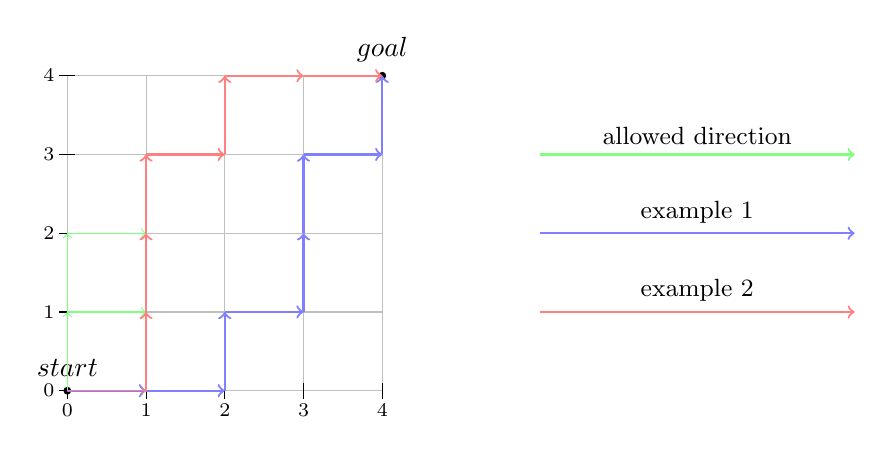
\begin{tikzpicture}
        \draw[color = gray!50] [] (0,0) grid (4,4);

        \foreach \c in {0,...,4}{
            \draw (\c,-.1) -- (\c,.1) node[below=4pt] {$\scriptstyle\c$};
            \draw (-.1,\c) -- (.1,\c) node[left=4pt] {$\scriptstyle\c$};
        }

        \node[label=above:$start$,style={fill, circle, inner sep = 1pt}] (A) at (0,0) {};
        \node[label=above:$goal$,style={fill, circle, inner sep = 1pt}] (Z) at (4,4) {};

        \draw[->, green!50, thick] (6,3) to node[above, midway, black] {\small{allowed direction}}  (10,3); 
        \draw[->, blue!50, thick]  (6,2) to node[above, midway, black] {\small{example 1}}           (10,2); 
        \draw[->, red!50, thick]   (6,1) to node[above, midway, black] {\small{example 2}}           (10,1); 

        \draw[->, green!50] (0,0) to (1,0);
        \draw[->, green!50] (0,0) to (0,1);
        \draw[->, green!50] (0,1) to (1,1);
        \draw[->, green!50] (0,1) to (0,2);
        \draw[->, green!50] (0,2) to (1,2);

        \draw[->, blue!50, thick] (0,0) to (1,0);
        \draw[->, blue!50, thick] (1,0) to (2,0);
        \draw[->, blue!50, thick] (2,0) to (2,1);
        \draw[->, blue!50, thick] (2,1) to (3,1);
        \draw[->, blue!50, thick] (3,1) to (3,2);
        \draw[->, blue!50, thick] (3,2) to (3,3);
        \draw[->, blue!50, thick] (3,3) to (4,3);
        \draw[->, blue!50, thick] (4,3) to (4,4);

        \draw[->, red!50, thin]  (0,0) to (1,0);
        \draw[->, red!50, thick] (1,0) to (1,1);
        \draw[->, red!50, thick] (1,1) to (1,2);
        \draw[->, red!50, thick] (1,2) to (1,3);
        \draw[->, red!50, thick] (1,3) to (2,3);
        \draw[->, red!50, thick] (2,3) to (2,4);
        \draw[->, red!50, thick] (2,4) to (3,4);
        \draw[->, red!50, thick] (3,4) to (4,4);
    \end{tikzpicture}
    \caption{Example for possible paths in a graph}
    \label{fig:example-paths-in-graph.tikz}
\end{figure}

\hint
The expression giving the number of different solutions contains factorials.  In order to get a better feeling
for the asymptotic growth of this expression we can use 
\href{https://en.wikipedia.org/wiki/Stirling%27s_approximation}{Stirling's approximation} of the factorial.
Stirling's approximation of $n!$ is given as follows: \index{Stirling's approximation of the factorial}
\\[0.2cm]
\hspace*{1.3cm}
$\ds n! \sim \sqrt{2 \cdot \pi \cdot n\,} \cdot \Bigl(\frac{n}{e}\Bigr)^n$.
\eox

\exercise
If there is no solution, the implementation of iterative deepening that is shown in Figure
\ref{fig:Iterative-Deepening.ipynb} does not terminate.  The reason is that the function $\texttt{dls}$ does not
distinguish between the following two reasons for failure:
\begin{enumerate}[(a)]
\item It can fail to find a solution because the depth limit is reached.
\item It can also fail because it has exhausted all possible paths without hitting the depth limit.
\end{enumerate}
Improve the implementation of iterative deepening so that it will always terminate eventually, provided the
state space is finite.
\eoxs


\section{Bidirectional Breadth First Search}
Breadth first search first visits all states that have a distance of 1 from start, then all
states that have a distance of 2, then of 3 and so on until finally the goal is found.  If the length of the shortest path
from $\texttt{start}$ to $\texttt{goal}$ is $d$, then all states that have a distance of at most $d$ will be
visited.  In many search problems, the number of states grows exponentially with the distance, i.e.~there is
a \blue{branching factor} $b$ \index{branching factor}
such that the set of all states that have a distance of at most $d$
from $\texttt{start}$ is roughly
\\[0.2cm]
\hspace*{1.3cm}
 $\ds 1 + b + b^2 + b^3 + \cdots + b^d = \frac{b^{d+1} - 1}{b - 1} = \mathcal{O}\bigl(b^d\bigr)$.
\\[0.2cm]
At least this is true in the beginning of the search.  As the size of
the memory that is needed is the most constraining factor when searching, it is important to cut down this
size.  If the search problem is \blue{symmetrical}, i.e.~if we have
\\[0.2cm]
\hspace*{1.3cm}
$x \in \mathtt{next\_states}(y) \;\Leftrightarrow\; y \in \mathtt{next\_states}(x)$,
\\[0.2cm]
then a simple idea is to start searching both from the node $\texttt{start}$ and the node $\texttt{goal}$
simultaneously.  This approach is known as \blue{bidirectional search}.  \index{bidirectional search}
All of the search problems that we have encountered so far are symmetrical.

The justification for bidirectional search is that the path starting from $\texttt{start}$ and the
path starting from $\texttt{goal}$ will meet in the middle and hence they will both have a size of approximately
$d/2$.  If this is the case, only
\\[0.2cm]
\hspace*{1.3cm}
$\ds 2 \cdot ( 1 + b + \cdots + b^{\frac{d}{2}} ) = 2 \cdot \frac{b^{\frac{d}{2}+1} - 1}{b - 1}$
\\[0.2cm]
nodes need to be explored and even for modest values of $b$ this number is much smaller than
\\[0.2cm]
\hspace*{1.3cm}
$\ds\frac{b^{d+1} - 1}{b - 1}$
\\[0.2cm]
which is the number of nodes expanded in breadth first search.  For example, assume that the branching factor
$b = 2$ and that the length of the shortest path leading from $\texttt{start}$ to $\texttt{goal}$
is $d = 40$.  Then we need to explore
\\[0.2cm]
\hspace*{1.3cm}
$2^{41} - 1 = 2,199,023,255,551$
\\[0.2cm]
states in breadth first search, while we only have to explore
\\[0.2cm]
\hspace*{1.3cm}
$2 \cdot \bigl(2^{\frac{40}{2}+1} - 1\bigr) = 4,194,302 $
\\[0.2cm]
states with bidirectional breadth first search.  While it is certainly feasible to keep four million states in memory,
keeping two trillion states in memory is impossible on most devices.  The
\myFig{example-area-usage-of-search.tikz} demonstrates that the conventional search algorithm has to use a lot
more space than the bidirectional approach. 

\begin{figure}[!ht]
    \centering
    \begin{subfigure}{.5\textwidth}
        \centering
        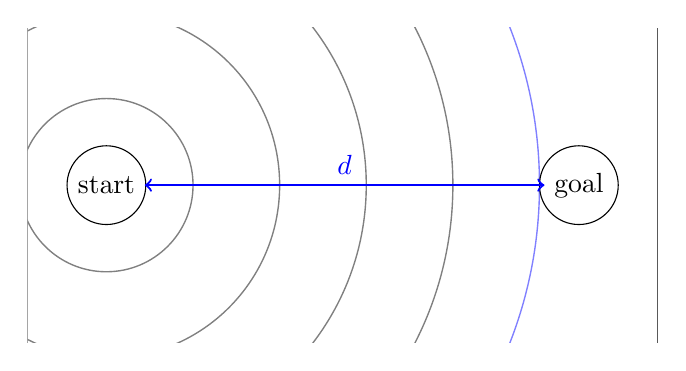
\begin{tikzpicture}
            \clip (0,0) rectangle + (8,4);
            \draw (0,0) -- (0,4);
            \draw (8,0) -- (8,4);

            \foreach \r in {1.1,2.2,...,4.4}{
                \draw[black!50, line width = 0.5pt] (1,2) circle (\r cm);
            }
            \draw[blue!50, line width = 0.5pt] (1,2) circle (5.5 cm);

            \draw (1,2) circle (0.5cm) node (A) {start};
            \draw (7,2) circle (0.5cm) node (B) {goal};

            \draw[<->, blue, thick] (A) to node[above, midway] {$d$} (B); 
        \end{tikzpicture}
        \caption{Conventional search}
        \label{fig:area-conventional-search.tikz}
    \end{subfigure}%
    \begin{subfigure}{.5\textwidth}
        \centering
        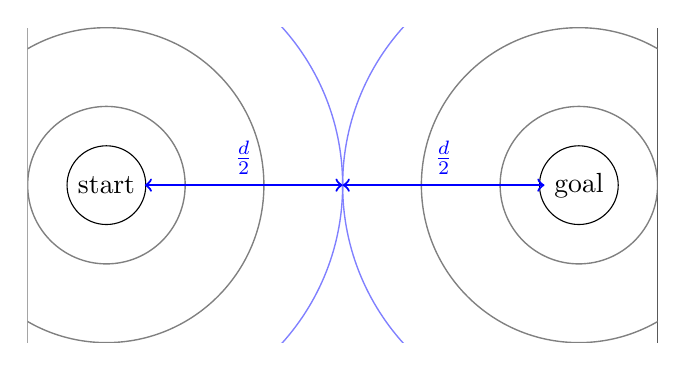
\begin{tikzpicture}
            \clip (0,0) rectangle + (8,4);
            \draw (0,0) -- (0,4);
            \draw (8,0) -- (8,4);

            \foreach \r in {1,2}{
                \draw[black!50, line width = 0.5pt] (1,2) circle (\r cm);
            }
            \draw[blue!50, line width = 0.5pt] (1,2) circle (3 cm);

            \foreach \r in {1,2}{
                \draw[black!50, line width = 0.5pt] (7,2) circle (\r cm);
            }
            \draw[blue!50, line width = 0.5pt] (7,2) circle (3 cm);

            \draw (1,2) circle (0.5cm) node (A) {start};
            \draw (7,2) circle (0.5cm) node (B) {goal};

            \draw[<->, blue, thick] (A) to node[above, midway] {$\frac{d}{2}$} (4,2); 
            \draw[<->, blue, thick] (B) to node[above, midway] {$\frac{d}{2}$} (4,2); 
        \end{tikzpicture}
        \caption{Bidirectional search}
        \label{fig:area-bidirectional-search.tikz}
    \end{subfigure}
    \caption{Example of space usage of conventional and bidrectional-BFS}
    \label{fig:example-area-usage-of-search.tikz}
\end{figure}


\begin{figure}[!ht]
\centering
\begin{python3code}
def search(start, goal, next_states):        
    FrontierA = { start }
    ParentA   = { start: start }
    FrontierB = { goal }
    ParentB   = { goal: goal } 
    while FrontierA and FrontierB:
        if Path := bfs_one_step(FrontierA, ParentA, ParentB, next_states):
            return Path
        if Path := bfs_one_step(FrontierB, ParentB, ParentA, next_states):
            return Path[::-1]
\end{python3code}
\vspace*{-0.3cm}
\caption{Bidirectional breadth first search.}
\label{fig:Bidirectional-BFS.ipynb}
\end{figure}

Figure \ref{fig:Bidirectional-BFS.ipynb} on page \pageref{fig:Bidirectional-BFS.ipynb} shows the implementation
of bidirectional breadth first search.  Essentially, we have two copies of the breadth first search program shown in
Figure \ref{fig:Breadth-First-Search.ipynb}.  However, since the information that was stored in the set
$\texttt{Visited}$ in the implementation of \textsc{bfs} shown in Figure \ref{fig:Breadth-First-Search.ipynb} is
also available in the dictionary $\texttt{Parent}$, we have removed the variable $\texttt{Visited}$ in our
implementation of bidirectional breadth first search.

Let us discuss the details of the implementation.
\begin{enumerate}
\item The variable $\texttt{FrontierA}$ is the frontier that starts from the state $\texttt{start}$, while
      $\texttt{FrontierB}$ is the frontier that starts from the state $\texttt{goal}$.
\item For every state $s$ that is in $\texttt{FrontierA}$, $\mathtt{ParentA}[s]$ is the state that caused $s$
      to be added to the set $\texttt{FrontierA}$.  Similarly, for every state $s$ that is in $\texttt{FrontierB}$,
      $\mathtt{ParentB}[s]$ is the state that caused $s$ to be added to the set $\texttt{FrontierB}$.
\item The bidirectional search keeps running for as long as both sets $\texttt{FrontierA}$ and
      $\texttt{FrontierB}$ are non-empty and a path has not yet been found. 
\item In line 7, the function \texttt{bfs\_one\_step} tries to compute a path that connects \texttt{start} with
      \texttt{goal}.  If such a path is found, this path which is then returned in
      line 8. 

      The details of the function \texttt{bfs\_one\_step} are discussed below.
\item Similarly, the function \texttt{bfs\_one\_step} in line 9 tries to find a path that connects \texttt{goal} with
      \texttt{start} by trying to expand states in \texttt{FrontierB}.
\end{enumerate}

\begin{figure}[!ht]
\centering
\begin{python3code}
def bfs_one_step(Frontier, ParentA, ParentB, next_states):
    NewFrontier = set()
    for s in Frontier:
        for ns in next_states(s):
            if ns not in ParentA:
                NewFrontier |= { ns }
                ParentA[ns]  = s
                if ns in ParentB:
                    return combinePaths(ns, ParentA, ParentB)
    Frontier.clear()
    Frontier.update(NewFrontier)
\end{python3code}
\vspace*{-0.3cm}
\caption{The function \texttt{bfs\_one\_step}.}
\label{fig:Bidirectional-BFS.ipynb-2}
\end{figure}

\noindent
The function \texttt{bfs\_one\_step} is shown in Figure \ref{fig:Bidirectional-BFS.ipynb-2} on page
\pageref{fig:Bidirectional-BFS.ipynb-2}.
\begin{enumerate}
\item The function \texttt{bfs\_one\_step} takes four arguments:
      \begin{enumerate}[(a)]
      \item \texttt{Frontier} is the frontier of states that result from a breadth first search
            that originates in a state $p$ where $p$ is either equal to \texttt{start} or to \texttt{goal}.
      \item \texttt{ParentA} is a dictionary.  For every state $q$ that is discovered in the breadth first
            search originating in $p$, $\mathtt{ParentA}[q]$ is a state that satisfies
            \\[0.2cm]
            \hspace*{1.3cm}
            $q \in \mathtt{next\_states}(\mathtt{ParentA}[q])$,
            \\[0.2cm]
            i.e.~$\texttt{ParentA}[q]$ is the state that lead to the state $q$.
      \item \texttt{ParentB} is a dictionary that is similar to \texttt{ParentA} but that instead contains
            as keys the states from the opposite search, i.e. if $p = \mathtt{start}$, then \texttt{ParentB}
            contains the states as keys that have been found while searching from \texttt{goal} and if instead
             $p = \mathtt{goal}$, then \texttt{ParentB} contains the states as keys that have been found while
             searching from \texttt{start}.
      \item For every state $s$, we have that $\texttt{next\_states}(s)$ is the set of states that can be
            reached in one step from $s$.
      \end{enumerate}
      The function \texttt{bfs\_one\_step} either returns a path or \texttt{None}.  In the latter case, the
      function just the set \texttt{Frontier} to contain those states that can be 
      reached in one step from the previous version of the set \texttt{Frontier}.  Hence, the function
      \texttt{bfs\_one\_step} performs one iteration of breadth first search.
\item The set \texttt{NewFrontier} is initialized as the empty set in line 2.
\item Next, we iterate over all states \texttt{s} in the set \texttt{Frontier}.
\item For every state \texttt{ns} that is reachable from the state \texttt{s} in one step and that has not
      already been visited, we add \texttt{ns} to the set \texttt{NewFrontier} in line 6 and record its
      parent in line 7.
\item If the state \texttt{ns} has already been reached in the search starting from \texttt{goal} and hence has
      a parent node in \texttt{ParentB}, we have found a path from start to goal.  Hence, We combine the path that
      leads from \texttt{start} to \texttt{ns} with the path leading from \texttt{goal} to \texttt{ns} in line 9.
\item It is important to note that the function \texttt{bfs\_one\_step} does not only return a path, it also
      has a side effect: If no path has been found, then the set \texttt{Frontier} is updated to contain those
      states that have been found in the current iteration.
\end{enumerate}
Finally, Figure \ref{fig:combine-paths.stlx} on page \pageref{fig:combine-paths.stlx} show the function
\texttt{combinePaths} that takes a \texttt{state} that is reachable from both \texttt{start} and \texttt{goal}.
It computes the path from \texttt{start} to the node \texttt{state} in line 2, the path from \texttt{goal} to
the node \texttt{state} in line 3 and then combines these paths by first reversing the second path and
appending it to the first path.  When combining the paths, we have to take care to remove the last state from
the first path \texttt{Path1}, since otherwise the node \texttt{state} would occur twice in the resulting path.

\begin{figure}[!ht]
\centering
\begin{python3code}
    def combinePaths(state, ParentA, ParentB):
            Path1 = path_to(state, ParentA)
            Path2 = path_to(state, ParentB)
            return Path1[:-1] + Path2[::-1] # Path2 is reversed
\end{python3code}
\vspace*{-0.3cm}
\caption{Combining two paths.}
\label{fig:combine-paths.stlx}
\end{figure}
On my computer, bidirectional breadth first search solves the $3 \times 3$ sliding puzzle in 81
milliseconds and uses 4 megabytes.  However, bidirectional breadth first search is still not able to solve the
more interesting cases of the $4 \times 4$ sliding puzzle since the portion of the search space that needs to
be computed is still too big to fit into memory. 

\section{Best First Search}
Up to now, all the search algorithms we have discussed have been essentially blind.  Given a state $s$ and
all of its neighbours, they had no idea which of the neighbours they should pick because they had no conception
which of these neighbours might be more promising than the other neighbours.  Search algorithms that know nothing
about the distance of a state to the goal are called \blue{blind}.  \index{blind search}
Russell and Norvig \cite{russell:2020} use the name \blue{uninformed search} instead of blind search.
\index{uninformed search} 

If a human tries to solve a search
problem, she will usually develop an intuition that certain states are more favourable than other states because
they seem to be closer to the solution.  In order to formalise this procedure, we next define the notion of a
\blue{search heuristic}. \index{search heuristic}

\begin{Definition}[Search Heuristic]
Given a search problem
\\[0.2cm]
\hspace*{1.3cm}
$\mathcal{P} = \langle Q, \mathtt{next\_states}, \mathtt{start}, \mathtt{goal} \rangle$,
\\[0.2cm]
a \blue{search heuristic} or simply \blue{heuristic} is a function \index{heuristic}
\\[0.2cm]
\hspace*{1.3cm}
$h: Q \rightarrow \mathbb{R}$
\\[0.2cm]
that computes an approximation of the distance of a given state $s$ to the state \texttt{goal}.
The heuristic is \blue{admissible} \index{admissible heuristic} if it never
\underline{\color{red}{overestimates}} the true distance, i.e.~if the function 
\\[0.2cm]
\hspace*{1.3cm}
$d:Q \rightarrow \mathbb{N}$
\\[0.2cm]
computes the \blue{true distance} from a state $s$ to the goal, then we must have
\\[0.2cm]
\hspace*{1.3cm}
$h(s) \leq d(s)$ \quad for all $s \in Q$.
\\[0.2cm]
Hence, the heuristic is admissible iff it is \blue{optimistic}: \index{optimistic heuristic}
Although it never overestimates the distance to the goal, it is free to underestimate this distance.

Finally, the  heuristic $h$ is called \blue{consistent} \index{consistent heuristic} iff we have 
\\[0.2cm]
\hspace*{1.3cm}
$h(\mathtt{goal}) = 0$ \quad and \quad $h(s_1) \leq 1 + h(s_2)$ \quad for all $s_2 \in \mathtt{next\_states}(s_1)$.  \eod
\end{Definition}

Let us explain the idea behind the notion of \blue{consistency}.  First, if we are already at the goal, the heuristic
should notice this fact and therefore we need to have $h(\mathtt{goal}) = 0$.  Secondly, assume we are at the state
$s_1$ and $s_2$ is a neighbour of $s_1$, i.e.~we have that
\\[0.2cm]
\hspace*{1.3cm}
$s_2 \in \mathtt{next\_states}(s_1)$.
\\[0.2cm]
Now if our heuristic $h$ assumes that the distance of $s_2$ from the $\texttt{goal}$ is $h(s_2)$, then the distance of
$s_1$ from the $\texttt{goal}$ can be at most $1 + h(s_2)$ because starting from $s_1$ we can first go to $s_2$
in one step and then from $s_2$ to $\texttt{goal}$ in $h(s_2)$ steps for a total of $1 + h(s_2)$ steps.  Of
course, it is possible that there exists a shorter path from $s_1$ leading to the $\texttt{goal}$ than the one
that visits $s_2$ first.  Hence, we have the inequality
\\[0.2cm]
\hspace*{1.3cm}
$h(s_1) \leq 1 + h(s_2)$.
\\[0.2cm]
The \myFig{demonstration-heuristic.tikz} demonstrates this inequality.

\begin{figure}[!ht]
    \centering
    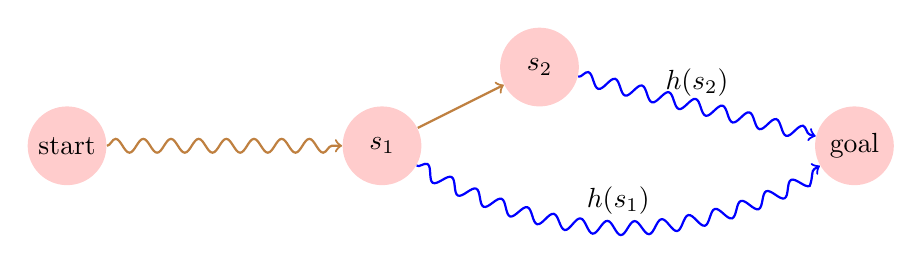
\begin{tikzpicture}
        \node (start)   at (0,0)   [circle, fill=red!20, inner sep=0pt, minimum size=1cm] {start};
        \node (s1)      at (4,0)   [circle, fill=red!20, inner sep=0pt, minimum size=1cm] {$s_1$};
        \node (s2)      at (6,1)   [circle, fill=red!20, inner sep=0pt, minimum size=1cm] {$s_2$};
        \node (goal)    at (10,0)  [circle, fill=red!20, inner sep=0pt, minimum size=1cm] {goal};

        \draw[->, thick, draw=brown, decorate, decoration=snake]   (start) to                                              (s1);
        \draw[->, thick, draw=brown]                               (s1)    to                                              (s2);
        \draw[->, thick, draw=blue, decorate, decoration=snake]    (s2)    to                node[midway,above] {$h(s_2)$} (goal);
        \draw[->, thick, draw=blue, decorate, decoration=snake]    (s1)    to[bend right=30] node[midway,above] {$h(s_1)$} (goal);
    \end{tikzpicture}
    \caption{Explanation of the inequality $h(s_1) \leq 1 + h(s_2)$.}
    \label{fig:demonstration-heuristic.tikz}
\end{figure}

\begin{Theorem}
  Every consistent heuristic is an admissible heuristic.
\end{Theorem}

\proof
Assume that the heuristic $h$ is consistent.  Assume further that $s \in Q$ is some state such that there is a
shortest path $P$ from $s$ to the $\texttt{goal}$.  Assume this path has the form
\\[0.2cm]
\hspace*{1.3cm}
$P = [s_n, s_{n-1}, \cdots, s_1, s_0]$, \quad where $s_n = s$ and $s_0 = \mathtt{goal}$.
\\[0.2cm]
Then the length of the path $p$ is $n$ and we have to show that $h(s) \leq n$.  In order to prove this claim, we show
that we have
\\[0.2cm]
\hspace*{1.3cm}
$h(s_k) \leq k$ \quad for all $k \in \{0, 1, \cdots, n\}$.
\\[0.2cm]
This claim is shown by induction on $k$.
\begin{enumerate}
\item[B.C.:] $k=0$.

             We have $h(s_0) = h(\mathtt{goal}) = 0 \leq 0$, because the fact that $h$ is consistent implies
             $h(\mathtt{goal}) = 0$.
\item[I.S.:] $k \mapsto k+1$.

             We have to show that $h(s_{k+1}) \leq k + 1$ holds.  This is shown as follows:
             \\[0.2cm]
             \hspace*{1.3cm}
             $
             \begin{array}[b]{lcll}
               h(s_{k+1}) & \leq & 1 + h(s_k) & \mbox{because $s_k \in \mathtt{next\_states}(s_{k+1})$ and $h$ is consistent,} \\[0.2cm]
                         & \leq & 1 + k      & \mbox{because $h(s_k) \leq k$ by induction hypotheses.} 
             \end{array}
             $ 
\end{enumerate}
We have shown $h(s_k) \leq k$ and since this also holds for $k = n$ we know that $h(s) = h(s_n) \leq n$.  Since $P$
is a shortest path we know that the state $s$ has the distance $n$ from the state $\texttt{goal}$.  Hence the
heuristic $h$ underestimates this distance and is therefore admissible.
\qed

It is natural to ask whether the last theorem can be reversed, i.e.~whether every admissible heuristic is also
consistent.  The answer to this question is negative since there are
some \emph{\color{red}contorted}\, heuristics that are admissible but that fail to be consistent.  However, in
practice it turns out that most 
admissible heuristics are also consistent.  Therefore, when we construct consistent heuristics later, we will
start with admissible heuristics, since these are easy to find.  We will then have to check that these
heuristics are also consistent.

\examples
In the following, we will discuss several heuristics for the sliding puzzle.
\begin{enumerate}
\item The simplest heuristic that is admissible is the function $h(s) := 0$.  Since we have
      \\[0.2cm]
      \hspace*{1.3cm}
      $0 \leq 1 + 0$,
      \\[0.2cm]
      this heuristic is obviously consistent, but when we use this heuristic, we are back to blind search.
\item The next heuristic is the \blue{number of misplaced tiles} heuristic.  For a state $s$,
      this heuristic counts the number of tiles in $s$ that are not in their final position, i.e.~that are not
      in the same position as the corresponding tile in $\texttt{goal}$.  For example, in \myFig{8-puzzle.pdf}
      in the state depicted to the left, only the tile with the label $4$ is in the same
      position as in the state depicted to the right.  Hence, there are 7 misplaced tiles.

      As every misplaced tile must be moved at least once and every step in the sliding puzzle moves at most
      one tile, it is obvious that this heuristic is admissible.  It is also consistent.  First, the
      $\texttt{goal}$ has no misplaced tiles, hence its heuristic is $0$.  Second, in every step of the sliding
      puzzle  only one tile is moved.  Therefore the number of misplaced tiles in two neighbouring states can
      differ by at most one and hence the inequality
      \\[0.2cm]
      \hspace*{1.3cm}
      $h(s_1) \leq 1 + h(s_2)$
      \\[0.2cm]
      is satisfied for any neighbouring states $s_1$ and $s_2$.  Unfortunately, the number of misplaced tiles
      heuristic is very crude and therefore not particularly useful.
\item The \blue{Manhattan heuristic} improves on the previous heuristic.  For two points
      $\pair(x_1, y_1), \pair(x_2, y_2) \in \mathbb{R}^2$ the \blue{Manhattan distance} of these
      points is defined as
      \\[0.2cm]
      \hspace*{1.3cm}
      $d_1\bigl(\langle x_1, y_1\rangle, \langle x_2, y_2\rangle\bigr) := |x_2 - x_1| + |y_2 - y_1|$.
      \\[0.2cm]
      The Manhattan distance is also called the \href{https://en.wikipedia.org/wiki/Taxicab_geometry}{$L_1$ norm}
      of the difference vector $\langle x_2 - x_1, y_2 - y_1 \rangle$.
      If we associate \href{https://en.wikipedia.org/wiki/Cartesian_coordinate_system}{Cartesian coordinates} with
      the tiles of the sliding puzzle such that the tile in the upper left corner has coordinates
      $\pair(1, 1)$ and the coordinates of the tile in the lower right corner are $\pair(3, 3)$, then
      the Manhattan distance of two positions measures how many steps it takes to move a tile from
      the first position to the second position if we are allowed to move the tile horizontally
      or vertically regardless of the fact that the intermediate positions might be blocked by
      other tiles.  To compute the Manhattan heuristic for a state $s$ with respect to the
      $\texttt{goal}$, we first define the function $\mathtt{pos}(t, s)$ for all tiles
      $t \in \{1,\cdots, 8\}$ in a given state $s$ as follows:
      \\[0.2cm]
      \hspace*{1.3cm}
      $\mathtt{pos}(t, s) = \pair(\mathtt{row}, \mathtt{col})
         \;\stackrel{\mathrm{def}}{\Longleftrightarrow}\; s[\mathtt{row}][\mathtt{col}] = t
      $,
      \\[0.2cm]
      i.e.~given a state $s$, the expression $\mathtt{pos}(t, s)$ computes the Cartesian coordinates of
      the tile $t$ with respect to the state $s$.  Then we can define the Manhattan heuristic $h$ for the $3
      \times 3$ puzzle 
      as follows:
      \\[0.2cm]
      \hspace*{1.3cm}
      $\ds h(s) := \sum\limits_{t=1}^8 d_1\bigl(\mathtt{pos}(t,s),\, \mathtt{pos}(t, \mathtt{goal})\bigr)$.
      \\[0.2cm]
      The Manhattan heuristic measures the number of moves that would be needed if we wanted to put every tile
      of $s$ into its final position and if we were allowed to slide tiles over each other.  Figure
      \ref{fig:manhattan.py} on page \pageref{fig:manhattan.py} shows how the Manhattan distance can be
      computed.  The code given in that figure works for a general $n \times n$ sliding puzzle.  It takes two
      states $\texttt{stateA}$ and $\texttt{stateB}$ and computes the Manhattan distance between these states.

      \begin{figure}[!ht]
        \centering
        \begin{minted}[ frame         = lines,
                          framesep      = 0.3cm,
                          firstnumber   = 1,
                          bgcolor       = sepia,
                          numbers       = left,
                          numbersep     = -0.2cm,
                          xleftmargin   = 0.8cm,
                          xrightmargin  = 0.8cm,
                        ]{python3}
    def manhattan(stateA, stateB):
        n = len(stateA)
        result = 0
        for rowA in range(n):
            for colA in range(n): 
                tile = stateA[rowA][colA]
                if tile != 0:
                    rowB, colB = find_tile(tile, stateB)
                    result += abs(rowA - rowB) + abs(colA - colB)
        return result
    \end{minted}
    \vspace*{-0.3cm}
    \caption{The Manhattan distance between two states.}
    \label{fig:manhattan.py}
    \end{figure}
    \FloatBarrier
    
      \begin{enumerate}
      \item First, the size $\texttt{n}$ of the puzzle is computed by checking the number of rows of
            $\texttt{stateA}$.
      \item Next, the \texttt{for} loops iterates over all rows and columns of $\texttt{stateA}$ that do not
            contain a blank tile.  Remember that the blank tile is coded using the number $0$.  The tile at
            position $\pair(\mathtt{rowA}, \mathtt{colA})$ in $\texttt{stateA}$ is computed using the expression \texttt{stateA[rowA][colA]} and the
            corresponding position $\pair(\mathtt{rowB}, \mathtt{colB})$ of this tile in state $\texttt{stateB}$ is computed using the function
            \texttt{find\_tile}.
      \item Finally, the Manhattan distance between the two positions $\pair(\mathtt{rowA}, \mathtt{colA})$ and
            $\pair(\mathtt{rowB}, \mathtt{colB})$ is added to the $\texttt{result}$.
      \end{enumerate}

    The Manhattan heuristic is admissible.  The reason is that if $s_2 \in \mathtt{next\_states}(s_1)$,
    then there can be only one tile $t$ such that the position of $t$ in $s_1$ is different from the position
    of $t$ in $s_2$.  Furthermore, this position differs by either one row or one column.  Therefore,
    \\[0.2cm]
    \hspace*{1.3cm}
    $|h(s_1) - h(s_2)| = 1$
    \\[0.2cm]
    and hence $h(s_1) \leq 1 + h(s_2)$.  \qed
\end{enumerate}
Now we are ready to present \blue{best first search}.  This algorithm is derived from the stack based
version of depth first search.  However, instead of using a stack, the algorithm uses a
\href{https://en.wikipedia.org/wiki/Priority_queue}{priority queue}.  In this priority queue, the paths are
ordered with respect to the estimated distance of the state at the end of the path from the $\texttt{goal}$.
We always expand the path next that seems to be closest to the goal.

In \textsl{Python} the module \href{https://docs.python.org/3.7/library/heapq.html}{\texttt{heapq}} provides 
\href{https://en.wikipedia.org/wiki/Priority_queue}{priority queues} that are implemented as 
\href{https://en.wikipedia.org/wiki/Heap_(data_structure)}{heaps}. 
Technically, these heaps are just lists.  In order to use them as priority queues, the entries of these lists
will be pairs of the form $(p, o)$, where $p$ is the priority of the object $o$.  Usually, the priorities are
numbers and, contra-intuitively, high priorities correspond to \textbf{small} numbers, that is $(p_1, o_1)$ has
a higher priority than $(p_2, o_2)$ if and only if $p_1 < p_2$. 
We need only two functions from the module \texttt{heapq}:
\begin{enumerate}
\item Given a heap $H$, the function $\texttt{heapq.heappop}(H)$ returns and removes the pair
      from H that has the highest priority.  
\item Given a heap $H$, the function $\texttt{heapq.heappush}\bigl(H, (p, o)\bigr)$  
      pushes the pair $(p, o)$ onto the heap $H$.  This method does not return a 
      value.  Instead, the heap $H$ is changed in place.
\end{enumerate}


\begin{figure}[!ht]
\centering
\begin{minted}[ frame         = lines,
                  framesep      = 0.3cm,
                  firstnumber   = 1,
                  bgcolor       = sepia,
                  numbers       = left,
                  numbersep     = -0.2cm,
                  xleftmargin   = 0.8cm,
                  xrightmargin  = 0.8cm,
                ]{python3}
    def search(start, goal, next_states, heuristic):
        Visited   = set()
        PrioQueue = [ (heuristic(start, goal), [start]) ]
        while PrioQueue:
            _, Path = heapq.heappop(PrioQueue)
            state   = Path[-1]
            if state == goal:
                return Path
            if state in Visited:
                continue
            for ns in next_states(state):           
                if ns not in Visited:
                    prio = heuristic(ns, goal)
                    heapq.heappush(PrioQueue, (prio, Path + [ns]))
            Visited.add(state)
\end{minted}
\vspace*{-0.3cm}
\caption{The best first search algorithm.}
\label{fig:Best-First-Search.ipynb}
\end{figure}

The function $\texttt{search}$ shown in \myFig{Best-First-Search.ipynb} takes four parameters.  The
first three of these parameters are the same as in the previous search algorithms.  The last parameter
$\texttt{heuristic}$ is a function that takes two states and then estimates the distance between these states.
Later, when solving the sliding puzzle, we will use the Manhattan distance to serve as the parameter
$\texttt{heuristic}$.  The details of the implementation are as follows:
\begin{enumerate}
\item The Variable \texttt{Visited} collects all states that have been \blue{visited}.  A node $n$ counts as
      \blue{visited} when all of its neighbours have been inspected in line 11.
\item The variable \texttt{PrioQueue} serves as a priority queue.  This priority queue is initialized as a
      list containing the pair $\langle d, [\mathtt{start}] \rangle$, where $d$ is the estimated distance of a path
      leading from \texttt{start} to \texttt{goal}.  In \texttt{PrioQueue} we store the paths 
      in pairs of the form
      \\[0.2cm]
      \hspace*{1.3cm}
      $\pair(\mathtt{estimate}, \mathtt{Path})$,
      \\[0.2cm]
      where $\texttt{Path}$ is a list of states starting from the node \texttt{start}.  If the last node on
      this list is called $\texttt{state}$, then we have
      \\[0.2cm]
      \hspace*{1.3cm}
      $\mathtt{estimate} = \mathtt{heuristic}(\mathtt{state}, \mathtt{goal})$,
      \\[0.2cm] 
      i.e.~\texttt{estimate} is the estimated distance between this \texttt{state} and \texttt{goal} and hence
      an estimate of the number of steps needed to complete \texttt{Path} into a solution.  This ensures,
      that the path whose last state is nearest to the \texttt{goal} is at the beginning of the set
      \texttt{PrioQueue}. 
\item As long as \texttt{PrioQueue} is not empty, we take the \texttt{Path} from the top of this
      priority queue and remove it from the queue.  This is then the path with the highest priority.
      If the state at the end of \texttt{Path} is named \texttt{state}, then \texttt{state} is, according to
      our heuristic, the state nearest to the \texttt{goal} among all states in the priority queue. 

      The function $\texttt{heappop}(\mathtt{PrioQueue})$ returns the smallest pair from 
      \texttt{PrioQueue} and, furthermore, this pair is removed from \texttt{PrioQueue}.
\item If \texttt{state} is the \texttt{goal}, a solution has been found and is returned.  
\item Next, we inspect all neighbouring states \texttt{ns} of \texttt{state} that have not already been
      visited.  The paths leading to these nodes are pushed on the priority queue.
\item Finally, we mark \texttt{state} as \blue{visited} by adding it to the set \texttt{Visited}.
\end{enumerate}
Best first search solves the instance of the $3 \times 3$ puzzle shown in \myFig{8-puzzle.pdf} in less than 3
millisecond and visits only 87 different states while solving the puzzle.  However, the solution that is found
takes 49 steps.  While the length of this solution is not as ridiculous as the length of the solution found by
depth first search,  this length is far from being optimal.  Best first search is able to solve the
$4 \times 4$ puzzle shown in \myFig{start-goal.stlx} in less than a second.  It visits 8224 different states in
order to find the solution.  Unfortunately, the solution that is found has a length of 492 steps, while the
optimal solution only needs 36 steps.

It should be noted that the fact that the Manhattan distance is a \blue{consistent} heuristic is of
no consequence for best first search.  Only the $\mathrm{A}^*$ algorithm, which is presented next, makes use of
this fact.

\section{A$^*$ Search \label{sec:a-star-search}}
We have observed that best-first search can be remarkably efficient. However, most of the times the solution it
provides is not optimal. This limitation arises because when best-first search considers a state \( s \), it
only takes into account the distance from \( s \) to the
\texttt{goal} state. Crucially, it neglects the distance from the \texttt{start} state to \( s \). In
contrast, the \blue{\(\mathrm{A}^*\) search algorithm} incorporates both the distance from \texttt{start} to
\(s \) and the estimated distance from \( s \) to the \texttt{goal}. As a result, when the heuristic employed
by the A\(^*\) search algorithm is admissible, it is assured to find the shortest path. 

Specifically, in the context of a given state \( s \), the function \( g(s) \) calculates the length of the
path from \texttt{start} to \( s \), and \( h(s) \) provides a heuristic estimate of the distance from \( s \)
to the \texttt{goal}. Consequently, the \blue{priority} utilized by the \(\mathrm{A}^*\) search algorithm is
expressed as 
\\[0.2cm]
\hspace*{1.3cm}
\( f(s) := g(s) + h(s) \).
\\[0.2cm]
The intricacies of the \(\mathrm{A}^*\) algorithm are detailed in \myFig{A-Star-Search.ipynb}.  When we compare
this implementation with the implementation of best first search shown in Figure
\ref{fig:Best-First-Search.ipynb} on page \pageref{fig:Best-First-Search.ipynb} we realize that these figure
differ only in line 13 where the priority of a path is computed.  With A$^*$ search, the priority of a path $P$
ending in state $s$ is the length of the path plus the estimated distance of the state $s$ to the
\texttt{goal}.  The fact that we have to add $1$ to $\mathtt{len}(\mathtt{Path})$ is due to the fact that
\texttt{Path} only leads to \texttt{state} and we need the length of the path that leads to \texttt{ns}.


\begin{figure}[!ht]
\centering
\begin{minted}[ frame         = lines,
                  framesep      = 0.3cm,
                  firstnumber   = 1,
                  bgcolor       = sepia,
                  numbers       = left,
                  numbersep     = -0.2cm,
                  xleftmargin   = 0.8cm,
                  xrightmargin  = 0.8cm,
                ]{python3}
    def search(start, goal, next_states, heuristic):
        Visited   = set()
        PrioQueue = [ (heuristic(start, goal), [start]) ]
        while PrioQueue:
            _, Path = heapq.heappop(PrioQueue)
            state   = Path[-1]
            if state in Visited:
                continue
            if state == goal:
                return Path
            for ns in next_states(state):           
                if ns not in Visited:
                    prio = len(Path) + heuristic(ns, goal)
                    heapq.heappush(PrioQueue, (prio, Path + [ns]))
            Visited.add(state)
\end{minted}
\vspace*{-0.3cm}
\caption{The A$^*$ search algorithm.}
\label{fig:A-Star-Search.ipynb}
\end{figure}
The $\mathrm{A}^*$ search algorithm has been discovered by Hart, Nilsson, and Raphael and was first published in
1968 \cite{hart:1968}.  However, there was a subtle bug in the first publication which was corrected
in 1972 \cite{hart:1972}.

When we run $\mathrm{A}^*$ search on the $3 \times 3$ sliding puzzle, it takes about $0.1$ seconds to solve the instance
shown in \myFig{8-puzzle.pdf} and visits 6614 states.
Furthermore, the good news about $\mathrm{A}^*$ search is that, provided the heuristic is admissible, the path which is
found is optimal \cite{hart:1972}.

\begin{Theorem}[Completeness and Optimality of $\mathrm{A}^*$ Search] \hspace*{\fill} \linebreak
  If $\mathcal{P} = \langle Q, \mathtt{next\_states}, \mathtt{start}, \mathtt{goal}\rangle$ is a search problem   and 
  $h: Q \rightarrow \mathbb{R}$ is a admissible heuristic for $\mathcal{P}$,
  then $\mathrm{A}^*$ search is both complete and optimal, i.e. if there is a path from start to goal, then
  the search is successful and, furthermore, the solution that is computed is a shortest path leading from 
  start to goal. 
\end{Theorem}

\proof
To simplify the notation of the proof we agree to use the following notation.
If $P$ is a path that is an element of \texttt{PrioQueue} and $s$ is the last state of the path $P$,
i.e.~$P[-1] = s$,  then we say that $s \in \mathtt{PrioQueue}$, although it really is the path $P$ that is an
element of \texttt{PrioQueue}.  Furthermore, we denote the length of $P$ with $g(s)$. Finally, we define
\\[0.2cm]
\hspace*{1.3cm}
$f(s) := g(s) + h(s)$  \quad for all the states $s \in \mathtt{PrioQueue}$. 
\\[0.2cm]
Therefore, $f(s)$ computes the priority of a state $s \in \mathtt{PrioQueue}$.

Next, the proof of our claim proceeds indirect.  We assume that the path $P_1 = [s_0, s_1, \cdots, s_n]$ that
is computed by $A^*$ search is not the shortest path.  Then there is a path $P_2 = [t_0, t_1, \cdots, t_m]$
leading from \texttt{start} to \texttt{goal} such that $P_2$ is shorter than $P_1$, i.e.~we must have $m < n$. 
We claim that 
\\[0.2cm]
\hspace*{1.3cm}
$f(t_i) \leq m$  \quad for all $i \in \{0, \cdots, m\}$.
\\[0.2cm]
The reasoning is as follows:
\\[0.2cm]
\hspace*{1.3cm}
$
\begin{array}[t]{lclr}
  f(t_i) & = & g(t_i) + h(t_i)  \\[0.2cm] 
         & = & i + h(t_i)     & \mbox{since $g(t_i) = \texttt{len}([t_0, \cdots, t_i]) = i$}  \\[0.2cm]
         & \leq & i + (m - i) & \mbox{since $h(t_i) \leq \texttt{len}([t_i, \cdots, t_m]) = m-i$} \\[0.2cm]
         & = & m                       
\end{array}
$
\\[0.2cm]
However, for the path $P_1$ we know that
\\[0.2cm]
\hspace*{1.3cm}
$f(s_n) = g(s_n) + h(s_n) = n + 0 = n > m$.
\\[0.2cm]
Since \texttt{PrioQueue} is a priority queue, we only remove the path $P_1$ from \texttt{PrioQueue} when all
paths with a higher priority have already been removed and the corresponding end notes have been
expanded.  But as $n > m$ this means that all paths
\\[0.2cm]
\hspace*{1.3cm}
$[t_0]$, $[t_0,t_1]$, $\cdots$, $[t_0, \cdots, t_m]$ 
\\[0.2cm]
have already been removed from \texttt{PrioQueue} before $P_1$ is removed.  But then $A^*$ search would have
already found the shortest path from \texttt{start} to \texttt{goal} and hence the path $P_1$ would never be
removed from \texttt{PrioQueue}.   This shows that $A^*$ search can't return a path that is not a shortest path.
\qed


\section{Bidirectional $\mathrm{A}^*$ Search}
\begin{figure}[!ht]
\centering
\begin{minted}[ frame         = lines,
                  framesep      = 0.3cm,
                  firstnumber   = 1,
                  bgcolor       = sepia,
                  numbers       = left,
                  numbersep     = -0.2cm,
                  xleftmargin   = 0.0cm,
                  xrightmargin  = 0.0cm,
                ]{python3}
    def search(start, goal, next_states, heuristic):
        VisitedA   = {}
        VisitedB   = {}
        PrioQueueA = [ (heuristic(start, goal), [start]) ]
        PrioQueueB = [ (heuristic(goal, start), [goal ]) ]
        while PrioQueueA and PrioQueueB:
            a, PathA = PrioQueueA[0]
            b, PathB = PrioQueueB[0]
            if a <= b:
                heapq.heappop(PrioQueueA)
                for Result in search_os(PrioQueueA, PathA, goal,
                                        VisitedA, VisitedB, next_states, heuristic):
                    return Result
            else:
                heapq.heappop(PrioQueueB)
                for Result in search_os(PrioQueueB, PathB, start,
                                        VisitedB, VisitedA, next_states, heuristic):
                    return Result[::-1]
    
    def search_os(PQ, Path, goal, VisitedA, VisitedB, next_states, heuristic):
        state = Path[-1]
        if state in VisitedA:
            return None
        if state in VisitedB:
            return Path[:-1] + VisitedB[state][::-1]
        for ns in next_states(state):           
            if ns not in VisitedA:
                prio1 = len(Path) + heuristic(ns, goal)
                prio2 = 2 * len(Path)
                prio  = max(prio1, prio2)
                heapq.heappush(PQ, (prio, Path + [ns]))
        VisitedA[state] = Path
\end{minted}
\vspace*{-0.3cm}
\caption{Bidirectional $\mathrm{A}^*$ search.}
\label{fig:Bidirectional-A-Star-Search.ipynb}
\end{figure}
\noindent
When we refined breadth first search into bidirectional breadth first search were able to increase the power of
breadth first search.  We can try to do something similar with the $\mathrm{A}^*$ algorithm and develop a
bidirectional variant of this algorithm.  \myFig{Bidirectional-A-Star-Search.ipynb} shows the resulting program.  This program
relates to the $\mathrm{A}^*$ algorithm shown in \myFig{A-Star-Search.ipynb} as the algorithm for bidirectional
search shown in \myFig{Bidirectional-BFS.ipynb} relates to breadth first search shown in \myFig{Breadth-First-Search.ipynb}.
The only new idea is that we alternate between the $\mathrm{A}^*$ search starting from $\texttt{start}$ and the
$\mathrm{A}^*$ search starting from $\texttt{goal}$ depending on the estimated total distance:
\begin{enumerate}[(a)]
\item As long as the search starting from $\texttt{start}$ is more promising, we remove states from
      \texttt{FrontierA}.
\item Once the total estimated distance of a path starting from $\texttt{goal}$ is less than the best total
      estimated distance of a path starting from $\texttt{start}$, we switch and remove states from $\texttt{FrontierB}$.
\end{enumerate}
There is one more twist, as the computation of the priority is a bit more involved.  This is necessary to
guarantee that the shortest path is computed.
    
When we run bidirectional $\mathrm{A}^*$ search for the $3 \times 3$ sliding puzzle shown in
\myFig{8-puzzle.pdf}, the program takes 150 milliseconds and uses $10,554$ states.  I have also
used bidirectional $A^*$ search to solve the $4 \times 4$ sliding puzzle shown in \myFig{start-goal.stlx}.  A
solution of $36$ steps was found in $2$ seconds. 
A total $77,870$ states had to be processed to compute this solution.
This shows that, counter-intuitively, bidirectional $A^*$ search uses more memory than unidirectional $A^*$
search.  Hence, in general, it not worth the trouble and we should stick with unidirectional $A^*$ search.




\begin{figure}[!ht]
\centering
\begin{Verbatim}[ frame         = lines,
                  framesep      = 0.3cm,
                  firstnumber   = 1,
                  labelposition = bottomline,
                  numbers       = left,
                  numbersep     = -0.2cm,
                  xleftmargin   = 0.8cm,
                  xrightmargin  = 0.8cm,
                ]
    start = ( (  0,  1,  2,  3 ),
              (  4,  5,  6,  8 ),
              ( 14,  7, 11, 10 ),
              (  9, 15, 12, 13 )
            )
    goal  = ( (  0,  1,  2,  3 ),
              (  4,  5,  6,  7 ),
              (  8,  9, 10, 11 ),
              ( 12, 13, 14, 15 )
            )
\end{Verbatim}
\vspace*{-0.3cm}
\caption{A start state and a goal state for the $4 \times 4$ sliding puzzle.}
\label{fig:start-goal.stlx}
\end{figure}
\pagebreak


\section{Iterative Deepening $\mathrm{A}^*$ Search \label{sec:ida-star-search}}
So far, we have combined $\mathrm{A}^*$ search with bidirectional search and achieved good results.  When
memory space is too limited for bidirectional $\mathrm{A}^*$ search to be possible, we can instead
combine $\mathrm{A}^*$ search with \blue{iterative deepening}.  The resulting search technique is known as
\href{https://en.wikipedia.org/wiki/Iterative_deepening_A*}{\color{blue}iterative deepening $\mathrm{A}^*$ search}
and is commonly abbreviated as  \textsc{ida} search.  \index{IDA$^*$ search}
It has been invented by Richard Korf \cite{korf:1985}.
 \myFig{iterative-deepening-a-star.stlx}
shows an implementation of \textsc{ida} search.  We proceed to discuss this program.

\begin{figure}[!ht]
\centering
\begin{minted}[ frame         = lines,
                  framesep      = 0.3cm,
                  firstnumber   = 1,
                  bgcolor       = sepia,
                  numbers       = left,
                  numbersep     = -0.2cm,
                  xleftmargin   = 0.0cm,
                  xrightmargin  = 0.0cm,
                ]{python3}
    def search(start, goal, next_states, heuristic):
        limit = heuristic(start, goal)
        while True:
            Path = dl_search([start], goal, next_states, limit, heuristic)
            if isinstance(Path, list):
                return Path
            limit = Path
    
    def dl_search(Path, goal, next_states, limit, heuristic):
        state    = Path[-1]
        distance = len(Path) - 1
        total    = distance + heuristic(state, goal)
        if total > limit:
            return total
        if state == goal:
            return Path
        smallest = float("Inf")  # infinity
        for ns in next_states(state):
            if ns not in Path:
                Solution = dl_search(Path+[ns], goal, next_states, limit, heuristic)
                if isinstance(Solution, list):
                    return Solution
                smallest = min(smallest, Solution)
        return smallest
\end{minted}
\vspace*{-0.3cm}
\caption{Iterative deepening $\textrm{A}^*$ search.}
\label{fig:iterative-deepening-a-star.stlx}
\end{figure}
\begin{enumerate}
\item As in the $\mathrm{A}^*$ search algorithm, the function \texttt{search} takes four parameters.
      \begin{enumerate}
      \item \texttt{start} is a state.  This state represents the start state of the search problem.
      \item \texttt{goal} is the goal state.
      \item \texttt{next\_states} is a function that takes a state $s$ as a parameter and
            computes the set of all those states that can be reached from $s$ in a single step.
      \item \texttt{heuristic} is a function that takes two parameters $s_1$ and $s_2$, where $s_1$ and $s_2$
            are states. The expression
            \\[0.2cm]
            \hspace*{1.3cm}
            $\texttt{heuristic}(s_1, s_2)$
            \\[0.2cm]
            computes an estimate of the distance between $s_1$ and $s_2$.  In \textsc{Ida} search it is required that this
            estimate is optimistic, i.e.~the \texttt{heuristic} has to be \blue{admissible}.
     \end{enumerate}
\item The function \texttt{search} initializes \texttt{limit} to be an estimate of the distance
      between \texttt{start} and \texttt{goal}.  As we assume that the function \texttt{heuristic} is
      optimistic, we know that there is no path from \texttt{start} to \texttt{goal} that is shorter than
      \texttt{limit}.  Hence, we start our search by assuming that we might find a path that has a length of
      \texttt{limit}.
\item Next, we start a \texttt{while} loop.  In this loop, we call the function \texttt{dl\_search} 
      (\blue{depth limited search}) to compute a path from
      \texttt{start} to \texttt{goal} that has a length of at most \texttt{limit}.  The function
      \texttt{dl\_search}  is described in detail below.
      When the function \texttt{dl\_search} returns, there are two cases:
      \begin{enumerate}
      \item \texttt{dl\_search} does find a path.  In this case, this path is returned in the variable
            \texttt{Path} and the value of this variable is a list.  This list is returned as the solution to
            the search problem.
      \item \texttt{dl\_search} is not able to find a path within the given \texttt{limit}.  In this case,
            \texttt{dl\_search} will not return a list representing a path, but instead it will return a number.
            This number will specify the minimal length that any path leading from \texttt{start} to \texttt{goal} needs to
            have.  This number is then used to update the \texttt{limit} which is used for the next
            invocation of \texttt{dl\_search}.

            \textbf{Note} that the fact that \texttt{dl\_search} is able to compute this new \texttt{limit} is
            a significant enhancement over iterative deepening.  While we had to test every single possible
            length in iterative deepening, now the fact that we can intelligently update the \texttt{limit}
            results in a considerable saving of computation time.
      \end{enumerate}
\end{enumerate}
We proceed to discuss the function \texttt{dl\_search}.  This function takes 5 parameters, which we describe next.
\begin{enumerate}
\item \texttt{Path} is a list of states.  This list starts with the state \texttt{start}.
      If \texttt{state} is the last state on this list, then \texttt{Path} represents a path leading from
      \texttt{start} to \texttt{state}.
\item \texttt{goal} is another state.  The purpose of the recursive invocations of \texttt{dl\_search} is to
      find a path from \texttt{state} to \texttt{goal}, where \texttt{state} is the last element of the
      list \texttt{Path}.
\item \texttt{next\_states} is a function that takes a state $s$ as input and computes the set of states that are
      reachable from $s$ in one step.
\item \texttt{limit} is the upper bound for the length of the path from \texttt{start} to \texttt{goal}.  If the
      function \texttt{dl\_search} is not able to find a path from \texttt{start} to \texttt{goal} that has
      a length of at most \texttt{limit}, then the search is unsuccessful.  In that case, instead of a path
      the function \texttt{dl\_search} returns a new estimate for the distance between \texttt{start} and
      \texttt{goal}.  Of course, this new estimate will be bigger than \texttt{limit}.
\item \texttt{heuristic} is a function taking two states as arguments.  The invocation
      $\texttt{heuristic}(s_1, s_2)$ computes an \blue{estimate} of the distance between the states $s_1$ and $s_2$.  It is
      assumed that this estimate is optimistic, i.e.~the value returned by $\texttt{heuristic}(s_1, s_2)$
      is less than or equal to the true distance between $s_1$ and $s_2$.
\end{enumerate}
We proceed to describe the implementation of the function \texttt{dl\_search}
\begin{enumerate}
\item The variable \texttt{state} is assigned the last element of \texttt{Path}.  Hence, \texttt{Path}
      connects \texttt{start} and \texttt{state}.
\item The length of the path connecting \texttt{start} and \texttt{state} is stored in 
      \texttt{distance}.
\item Since \texttt{heuristic} is assumed to be optimistic,  if we want to extend \texttt{Path}, then the best we
      can hope for is to find a path from \texttt{start} to \texttt{goal} that has a length of
      \\[0.2cm]
      \hspace*{1.3cm}
      $\texttt{distance} + \texttt{heuristic}(\texttt{state}, \texttt{goal})$.
      \\[0.2cm]
      This length is computed and saved in the variable \texttt{total}.
\item If \texttt{total} is bigger than \texttt{limit}, it is not possible to find a path from
      \texttt{start} to \texttt{goal} passing through \texttt{state} that has a length of at most
      \texttt{limit}.  Hence, in this case we return \texttt{total} to communicate that the limit needs to
      be increased to have at least a value of \texttt{total}.
\item If we are lucky and \texttt{state} is equal to \texttt{goal}, the search is successful and \texttt{Path}
      is returned. 
\item Otherwise, we iterate over all nodes \texttt{ns} reachable from \texttt{state} that have not already been visited
      by \texttt{Path}.  If \texttt{ns} is a node of this kind, we extend the \texttt{Path} so that
      this node is visited next.  The resulting path has the form
      \\[0.2cm]
      \hspace*{1.3cm}
      \texttt{Path + [ns]}.
      \\[0.2cm]
      Next, we recursively start a new search starting from the node \texttt{ns}.  If this search is
      successful, the resulting path is returned.  Otherwise, the search returns the minimum distance that is
      needed to reach the state \texttt{goal} from the state \texttt{start} on a path via the state
      \texttt{ns}.  If this distance is smaller than the distance \texttt{smallest} that is returned from
      visiting previous neighbouring nodes, the variable \texttt{smallest} is updated accordingly.
      This way, if the \texttt{for} loop is not able to return a path leading to \texttt{goal}, the variable
      \texttt{smallest} contains a lower bound for the distance that is needed to reach \texttt{goal} by a path that
      extends the given \texttt{Path}. 

      \textbf{Note}: At this point, a natural question is to ask whether the $\texttt{for}$ loop should collect
      all paths leading to \texttt{goal} and then only return the path that is shortest.  However, this is
      not necessary:  Every time the function \texttt{dl\_search} is invoked it is already guaranteed that there
      is no path that is shorter than the parameter \texttt{limit}.  Therefore, if \texttt{dl\_search} is able
      to find a path that has a length of at most \texttt{limit}, this path is known to be optimal.
\end{enumerate}
Iterative deepening $\mathrm{A}^*$ is a complete search algorithm that does find an optimal path, provided that the employed heuristic
is optimistic.  On the instance of the $3 \times 3$ sliding puzzle shown on \myFig{8-puzzle.pdf}, this
algorithm takes about $1.2$ seconds to solve the puzzle.  Only about 170 kilobytes of memory are necessary for
this search.  For the $4 \times 4$ sliding puzzle shown in Figure
\ref{fig:start-goal.stlx}, the algorithm 
takes about $1.6$ seconds and uses 184 kilobytes.  Although this is more than the time needed by bidirectional $\mathrm{A}^*$ search,
the good news is that the $\mathrm{IDA}^*$ algorithm does not need much memory since basically only the path
discovered so far is stored in memory.  Hence, $\mathrm{IDA}^*$ is a viable alternative if the available memory
is not sufficient to support the bidirectional $\mathrm{A}^*$ algorithm.

% \section{$\mathrm{A}^*$-$\mathrm{IDA}^*$ Search}
% So far, of all the search algorithms we have tried, the bidirectional $\mathrm{A}^*$ search has performed best.  However,
% bidirectional $\mathrm{A}^*$ search is only feasible if sufficient memory is available.   While
% $\mathrm{IDA}^*$ requires more time, its memory consumption is much lower than the memory consumption of
% bidirectional $\mathrm{A}^*$.  Hence, it is natural to try to combine the $\mathrm{A}^*$ algorithm and the
% $\mathrm{IDA}^*$ algorithm.  Concretely, the
% idea is to run an $\mathrm{A}^*$ search from the $\texttt{start}$ node until memory is more or less
% exhausted.  Then, we start $\mathrm{IDA}^*$ from the $\texttt{goal}$ node and search until we find any of the
% nodes discovered by the $\mathrm{A}^*$ search that had been started from the $\texttt{start}$ node.
% \index{A$^*$-IDA$^*$ search}


% \begin{figure}[!ht]
% \centering
% \begin{minted}[ frame         = lines,
%                   framesep      = 0.3cm,
%                   firstnumber   = 1,
%                   bgcolor       = sepia,
%                   numbers       = left,
%                   numbersep     = -0.2cm,
%                   xleftmargin   = 0.0cm,
%                   xrightmargin  = 0.0cm,
%                 ]{python3}
%     def search(start, goal, next_states, heuristic, size):
%         Parent   = { start:start }
%         Distance = { start: 0 }           
%         estGoal  = heuristic(start, goal)
%         Estimate = { start: estGoal }
%         Frontier = Set()
%         Frontier.insert( (estGoal, start) )
%         while len(Distance) < size and Frontier:
%             estimate, state = Frontier.pop()
%             if state == goal:
%                 return path_to(state, Parent)
%             stateDist = Distance[state]
%             for ns in next_states(state):
%                 oldEstimate = Estimate.get(ns, None)
%                 newEstimate = stateDist + 1 + heuristic(ns, goal)
%                 if oldEstimate is None or newEstimate < oldEstimate:
%                     Distance[ns] = stateDist + 1
%                     Estimate[ns] = newEstimate
%                     Parent[ns]   = state
%                     Frontier.insert( (newEstimate, ns) )
%                     if oldEstimate is not None:
%                         Frontier.delete( (oldEstimate, ns) )
%         Path = id_search(goal, start, next_states, heuristic, Distance)
%         return path_to(Path[-1], Parent) + Path[::-1][1:]
% \end{minted}
% \vspace*{-0.3cm}
% \caption{The $\mathrm{A}^*$-$\mathrm{IDA}^*$ search algorithm, part \texttt{I}.}
% \label{fig:A-Star-Ida-Star.ipynb-1}
% \end{figure}

% An implementation of the $\mathrm{A}^*$-$\mathrm{IDA}^*$ algorithm is shown in \myFig{A-Star-Ida-Star.ipynb-1}
% and \myFig{A-Star-Ida-Star.ipynb-2}.  We begin with a discussion of the function $\texttt{search}$.
% \begin{enumerate}
% \item The function $\texttt{search}$ takes 5 arguments.
%       \begin{enumerate}[(a)]
%       \item $\texttt{start}$ and $\texttt{goal}$ are states.  The function tries to find a path connecting
%             $\texttt{start}$ and $\texttt{goal}$.
%       \item $\texttt{next\_states}$ is a function that takes a state $s$ as input and computes the set of states that are
%             reachable from $s$ in one step.
%       \item $\texttt{heuristic}$ computes an \blue{estimate} of the distance between $s_1$ and $s_2$.  It is
%             assumed that this estimate is both \blue{admissible} and \blue{consistent}.
%       \item $\texttt{size}$ is the maximal number of states that the $\mathrm{A}^*$ search is allowed to
%             explore before the algorithm switches over to $\mathrm{IDA}^*$ search.
%       \end{enumerate}
% \item The basic idea behind the $\mathrm{A}^*$-$\mathrm{IDA}^*$ algorithm is to first use $\mathrm{A}^*$ search
%       to find a path from $\texttt{start}$ to $\texttt{goal}$.  If this is successfully done without visiting
%       more than $\texttt{size}$ nodes, the algorithm terminates and returns the path that has been found.
%       Otherwise, the algorithm switches over to an $\mathrm{IDA}^*$ search that starts from $\texttt{goal}$ and
%       tries to connect goal to any of the nodes that have been encountered during the $\mathrm{A}^*$ search.
%       To this end, the function $\texttt{search}$ maintains the following variables.
%       \begin{enumerate}
%       \item $\texttt{Parent}$ is a dictionary associating a parent state with those states that have already been
%             encountered during the search, i.e.~we have
%             \\[0.2cm]
%             \hspace*{1.3cm}
%             $\texttt{Parent}[s_2] = s_1 \;\Rightarrow\; s_2 \in \texttt{next\_states}(s_1)$.
%             \\[0.2cm]
%             Once the goal has been found, this dictionary is used to compute the path from $\texttt{start}$ to
%             $\texttt{goal}$.
%       \item $\texttt{Distance}$ is a dictionary that remembers for every state $s$ that is encountered during the
%             $\mathrm{A}^*$ search the length of the shortest path from $\texttt{start}$ to $s$.
%       \item $\texttt{Estimate}$ is a dictionary.  For every state $s$ encountered in the $\mathrm{A}^*$ search, $\texttt{Estimate}[s]$
%             is an estimate of the length that a path from $\texttt{start}$ to $\texttt{goal}$ would have if it would
%             pass through the state $s$.  This estimate is calculated using the equation
%             \\[0.2cm]
%             \hspace*{1.3cm}
%             $\texttt{Estimate}[s] = \texttt{Distance}[s] + \texttt{heuristic}(s, \texttt{goal})$.
%             \\[0.2cm]
%             Instead of recalculating this sum every time we need it, we store the sum in the dictionary
%             $\texttt{Estimate}$.
%       \item $\texttt{Frontier}$ is a \href{https://en.wikipedia.org/wiki/Priority_queue}{priority queue}.
%             The elements of $\texttt{Frontier}$ are pairs of the form
%             \\[0.2cm]
%             \hspace*{1.3cm}
%             $(d, s)$ \quad such that \quad $d = \texttt{Estimate}[s]$,
%             \\[0.2cm]
%             i.e.~if $(d, s) \in \texttt{Frontier}$, then the state $s$ has been encountered in the $\mathrm{A}^*$ search and it is
%             estimated that a path leading from $\texttt{start}$ to $\texttt{goal}$ and passing through $s$ would have
%             a length of $d$.  This priority queue is implemented as an ordered set.
%       \end{enumerate}
% \item The $\mathrm{A}^*$ search runs exactly as discussed in section \ref{sec:a-star-search}.  The only difference is that the
%       \texttt{while} loop is terminated once the dictionary $\texttt{Distance}$ has more than $\texttt{size}$
%       entries.  If we are lucky, the $\mathrm{A}^*$ search is already able to find the $\texttt{goal}$ and the
%       algorithm terminates.
% \item Otherwise, the function $\texttt{id\_search}$ is called.  This function starts an iterative deepening
%   $\mathrm{A}^*$ search from the node $\texttt{goal}$.  This works as described in section \ref{sec:ida-star-search}.
%       This search terminates as soon as a state is found
%       that has already been encountered during the $\mathrm{A}^*$ search.  The set of these nodes is given to
%       the function $\texttt{id\_search}$ via the dictionary $\texttt{Distance}$.  The function
%       $\texttt{id\_search}$ returns a path leading from $\texttt{goal}$ to a state $s$ that is a key of the
%       dictionary $\texttt{Distance}$ and hence has been reached by the  A$^*$ search. 
%       In order to compute a path from $\texttt{start}$ to $\texttt{goal}$, we still have to compute a
%       path from $\texttt{start}$ to $s$.  This path is then combined with the path $\texttt{P}$ and the resulting path
%       is returned.

%       The expression \texttt{Path[::-1]} in line 24 reverses the list $\texttt{Path}$ and 
%       hence \texttt{Path[::-1]} is a path leading from the state $s$ to the state $\texttt{goal}$.
%       \texttt{Path[::-1][-1]} is the same path but without the state $s$, as this state is already included 
%       as the last state of the path returned by the expression
%       \\[0.2cm]
%       \hspace*{1.3cm}
%       \texttt{path\_to(Path[-1], Parent)}.
% \end{enumerate}


% \begin{figure}[!ht]
% \centering
% \begin{minted}[ frame         = lines,
%                   framesep      = 0.3cm,
%                   firstnumber   = 1,
%                   bgcolor       = sepia,
%                   numbers       = left,
%                   numbersep     = -0.2cm,
%                   xleftmargin   = 0.0cm,
%                   xrightmargin  = 0.0cm,
%                 ]{python3}
%     def id_search(goal, start, next_states, heuristic, Distance):
%         limit = 0
%         while True:
%             Path = dl_search([goal], start, next_states, limit, heuristic, Distance)
%             if isinstance(Path, list):
%                 return Path
%             limit = Path
    
%     def dl_search(Path, start, next_states, limit, heuristic, Distance):
%         state = Path[-1]
%         total = len(Path) - 1 + heuristic(state, start)
%         if total > limit:
%             return total
%         if state in Distance:
%             return Path
%         smallest = float('Inf')
%         for ns in next_states(state):
%             if ns not in Path:
%                 result = dl_search( Path + [ns], start, next_states, limit, 
%                                     heuristic, Distance
%                                   )
%                 if isinstance(result, list):
%                     return result
%                 smallest = min(smallest, result)
%         return smallest 
% \end{minted}
% \vspace*{-0.3cm}
% \caption{The $\mathrm{A}^*$-$\mathrm{IDA}^*$ search algorithm, part \texttt{II}.}
% \label{fig:A-Star-Ida-Star.ipynb-2}
% \end{figure}

% Iterative deepening $\mathrm{A}^*$-$\mathrm{IDA}^*$ is a complete search algorithm.
% On the instance of the $3 \times 3$ sliding puzzle shown on \myFig{8-puzzle.pdf}, this
% algorithm takes about $0.14$ seconds to solve the puzzle.  For the $4 \times 4$ sliding puzzle, if the algorithm
% is allowed to visit at most $3\,000$ states, the algorithm takes less than $1.33$ seconds.
%  $\mathrm{A}^*$-$\mathrm{IDA}^*$ is not optimal.  For example the solution computed for 
% the $4 \times 4$ sliding puzzle has a length of 40, while the shortest solution for the given problem only
% requires 36 steps.


\exercise
The \href{https://en.wikipedia.org/wiki/Eight_queens_puzzle}{eight queens puzzle} is the problem of  placing
eight chess queens on a chessboard so that no two queens can attack each other.  In
\href{https://en.wikipedia.org/wiki/Chess}{chess}, a \href{https://en.wikipedia.org/wiki/Queen_(chess)}{queen}
can attack by moving horizontally, vertically, or diagonally.  
\begin{enumerate}[(a)]
\item Reformulate the \blue{eight queens puzzle} as a search problem.
\item Compute an upper bound for the number of states.
\item Which of the algorithms we have discusses are suitable to solve this problem?
\item Compute all 92 solutions of the eight queens puzzle.  
\end{enumerate}

\hint
It is easiest to encode states as lists.  For example, the solution of the eight queens puzzle that is shown in
Figure \ref{fig:queens.pdf} would be represented as the list 
\\[0.2cm]
\hspace*{1.3cm}
$[6, 4, 7, 1, 8, 2, 5, 3]$
\\[0.2cm]
because the queen in the first row is positioned in column 6, the queen in the second row is positioned in
column 4, and so on.  The start state would then be the empty list and given a state $L$, all states from the
set $\mathtt{nextState}(L)$ would be lists of the form $L + [c]$.  If $\#L = k$, then the state $l + [c]$ has
$k+1$ queens, where the queen in row $k+1$ has been placed in column $c$.
A frame for solving this problem is available at
\href{https://github.com/karlstroetmann/Artificial-Intelligence/blob/master/Python/1
  Search/14-N-Queens.ipynb}{Artificial-Intelligence/blob/master/Python/1 Search/14-N-Queens.ipynb}.


\begin{figure}[!ht]
\centering
\epsfig{file=Figures/queens.pdf},
\caption{A solution of the eight queens puzzle.}
\label{fig:queens.pdf}
\end{figure}
\pagebreak
\vspace*{1cm}


\exercise
The founder of \href{https://en.wikipedia.org/wiki/Taoism}{Taoism}, the Chinese philosopher
\href{https://en.wikipedia.org/wiki/Laozi}{Laozi} once said:
\\[0.2cm]
\hspace*{1.3cm}
\textsl{``A journey of a thousand miles begins but with a single step''}.
\\[0.2cm]
This proverb is the foundation of \blue{taoistic search}.  The idea is, instead of trying to reach
the goal directly, we rather define some intermediate states which are easier to reach than the goal state and
that are nearer to the goal than the start state.  To make this idea more precise, consider the following instance of the
15-puzzle, where the states $\texttt{Start}$ and $\texttt{Goal}$ are given as follows:
\begin{verbatim}
        Start :=  +---+---+---+---+    Goal :=  +---+---+---+---+
                  |   |15 |14 | 8 |             |   | 1 | 2 | 3 |
                  +---+---+---+---+             +---+---+---+---+
                  |12 |10 |11 |13 |             | 4 | 5 | 6 | 7 |
                  +---+---+---+---+             +---+---+---+---+
                  | 9 | 6 | 2 | 5 |             | 8 | 9 |10 |11 |
                  +---+---+---+---+             +---+---+---+---+
                  | 1 | 3 | 4 | 7 |             |12 |13 |14 |15 |
                  +---+---+---+---+             +---+---+---+---+
 \end{verbatim}
 In order to solve this instance of the 15-puzzle, we could try to first move the tiles numbered with $14$ and
 $15$ into the lower right  corner.  The resulting state would have the following form:
 \begin{verbatim}
                  +---+---+---+---+
                  | * | * | * | * |
                  +---+---+---+---+
                  | * | * | * | * |
                  +---+---+---+---+
                  | * | * | * | * |
                  +---+---+---+---+
                  | * | * |14 |15 |
                  +---+---+---+---+
 \end{verbatim}
 Here, the character ``\texttt{*}'' is used as a wildcard character, i.e.~we do not care about the actual
 character in the state, for we only want to ensure that the first two tiles are positioned correctly.  Once we have reached a
 state specified by the pattern given above, we could then proceed to reach a state that is described by the
 following pattern:


 \begin{verbatim}
                  +---+---+---+---+
                  | * | * | * | * |
                  +---+---+---+---+
                  | * | * | * | * |
                  +---+---+---+---+
                  | * | * | * | * |
                  +---+---+---+---+
                  |12 |13 |14 |15 |
                  +---+---+---+---+
 \end{verbatim}
 We have now solved the bottom line of the puzzle.  In a similar way, we can try to solve the line above the
 bottom line.  After that, the next step would be to reach a goal of the form
 \begin{verbatim}
                  +---+---+---+---+
                  | * | * | 2 | 3 |
                  +---+---+---+---+
                  | * | * | 6 | 7 |
                  +---+---+---+---+
                  | 8 | 9 |10 |11 |
                  +---+---+---+---+
                  |12 |13 |14 |15 |
                  +---+---+---+---+
\end{verbatim}
The final step would then solve the puzzle.  I have prepared a framework for taoistic search.  The file
\\[0.2cm]
\hspace*{1.5cm}
\href{https://github.com/karlstroetmann/Artificial-Intelligence/blob/master/Python/1%20Search/15-Taoistic-Search.ipynb}{\texttt{Python/1 Search/15-Taoistic-Search.ipynb}}
\\[0.2cm]
from my github repository at
\href{https://github.com/karlstroetmann/Artificial-Intelligence/}{\texttt{https://github.com/karlstroetmann/Artificial-Intelligence}} \linebreak
contains a framework to solve the sliding puzzle using taoistic search where some functions are left unimplemented.  
 Your task is to implement the missing functions in this file and thereby solve the puzzle.
 \eox

%%% Local Variables:
%%% mode: latex
%%% TeX-master: "artificial-intelligence"
%%% eval: (setenv "LANG" "en_US.UTF-8")
%%% End:
